\chapter{Two-dimensional finite-volume methods}
\label{chp-2d-fv}
In Chapter \ref{chp-1d-fv}, we addressed the problem of solving the one-dimensional
linear advection equation using the finite-volume method based on PPM. In this chapter, our focus shifts to solving the two-dimensional 
linear advection equation using the finite-volume method. This step is crucial in our work since, as we will explore in Chapter 
\ref{chp-cs-fv}, solving the linear advection equation on the cubed-sphere relies on solving two-dimensional linear advection equations 
at each cube face, with interpolation between adjacent panels.

A natural approach to develop a finite-volume method for the two-dimensional linear advection equation would involve extending PPM to 
two dimensions. Indeed, \citet{rancic:1992} proposed a piecewise bi-parabolic extension of PPM using a semi-Lagrangian temporal 
discretization. 
Further, this type of method can be extended to the cubed-sphere \citep{lauritzen:2010}.
However, this method suffers from a significant drawback—its computationally expensive nature. As a popular alternative, 
dimension-splitting methods are often used, which replace the two-dimensional problem with a sequence of one-dimensional problems. For 
example, we can solve the two-dimensional linear advection equation by solving a series of one-dimensional linear advection equations 
using the PPM from Chapter \ref{chp-1d-fv}. Moreover, in principle, we can employ any numerical method that solves the one-dimensional 
linear advection equation.

A comparison between two-dimensional and dimension-splitting semi-Lagrangian schemes on a plane was investigated by \citet{chen:2017}, 
utilizing the PPM as the one-dimensional solver and distorted two-dimensional grids. Their main conclusion was that dimension-splitting 
schemes are more sensitive to grid distortions, but they are computationally cheaper and more accurate than two-dimensional methods, 
particularly when dealing with large CFL numbers.

The primary objective of this chapter is to provide a comprehensive explanation of the dimension splitting method proposed by 
\citet{lin:1996}. This method is currently utilized in the FV3 dynamical core and is applied to the two-dimensional linear advection 
equation using the one-dimensional finite-volume schemes described in Chapter \ref{chp-1d-fv}.
Similar to Chapter \ref{chp-1d-fv}, we start this chapter with a review of the integral form of the two-dimensional advection 
equation in Section \ref{sec-adv2d}. In Section \ref{sec:fv-2d}, we establish the framework for general two-dimensional finite-volume 
schemes. The dimension splitting method is presented in Section \ref{sec-dsplit}, and we showcase numerical experiments in Section 
\ref{sec-ds-exp}.
\section{Two-dimensional advection equation in integral form}
\label{sec-adv2d}

\subsection{Notation}
\label{chp3-sec-not}
This section is dedicated to extending the notation of Section \ref{chp2-sec-not}.
Based on definitions \ref{chp2-def-dxgrid} and \ref{chp2-def-dxtimegrid},
we introduce the concepts of a $(\Delta x,\Delta y)$-grid and $(\Delta x, \Delta y, \Delta t, \lambda)$ discretization.
Throughout this chapter, we will use the notation $\Omega=[a,b]\times[c,d]$
and $\nu$ to represent a non-negative integer indicating the number of ghost cell layers in each boundary.
We also use the notations $\mathbb{R}^{N\times M}_{\nu}:=\mathbb{R}^{(N+2\nu)\times (M+2\nu)}$ and
$\mathbb{R}^{(N+1)\times M}_{\nu}:=\mathbb{R}^{(N+1+2\nu)\times (M+2\nu)}$,
$\mathbb{R}^{N\times (M+1)}_{\nu}:=\mathbb{R}^{(N+2\nu)\times (M+1+2\nu)}$.
\begin{definition}[$(\Delta x,\Delta y)$-grid]
	\label{chp2-def-2dgrid}
	Given $\Omega$ and positive real numbers $\Delta x$ and $\Delta y$ such that $\Delta x = (b-a)/N$, 
	$\Delta y = (d-c)/M$, for positive integers $N$ and $M$,
	we say that $\Omega_{\Delta x, \Delta y}=(\Omega_{ij})_{i=-\nu+1,\ldots,N+\nu}^{j=-\nu+1,\ldots,M+\nu}$
	is a $(\Delta x, \Delta y)$-grid for $\Omega$ if
    \begin{equation*}
	\Omega_{ij} = [x_{i-\frac{1}{2}}, x_{i+\frac{1}{2}}]\times [y_{j-\frac{1}{2}}, y_{j+\frac{1}{2}}] =
    [a+(i-1)\Delta x,a+i\Delta x]\times [c+(j-1)\Delta x,c+j\Delta x],
    \end{equation*}
	$\Delta x = x_{i+\frac{1}{2}}-x_{i-\frac{1}{2}}$, 	$\Delta y = y_{j+\frac{1}{2}}-y_{j-\frac{1}{2}}$.
	Each $\Omega_{ij}$ is called control volume or cell.
	The cell centroids $(x_i,y_j)$ are defined by
    \begin{align*}
       x_i = \frac{1}{2}(x_{i+\frac{1}{2}} + x_{i-\frac{1}{2}}), y_j = \frac{1}{2}(y_{j+\frac{1}{2}} + y_{j-\frac{1}{2}}).
    \end{align*}
\end{definition}
\begin{remark}
If $1 \leq i \leq N$,$1 \leq j \leq M$, we refer to $(i,j)$ as an interior index;
otherwise, $(i,j)$ is considered a ghost cell index and we say the $\Omega_{ij}$ is a ghost cell.
\end{remark}
\begin{definition}[$(\Delta x,\Delta y,\Delta t, \lambda)$-discretization]
	\label{chp2-def-dxdytimegrid}
	Given $\Omega \times [0,T]$,
	and positive real numbers $\Delta x$ $\Delta y$ and $\Delta t$, we say that
	$(\Omega_{\Delta x, \Delta y}, {T}_{\Delta t})$
	is a $(\Delta x,\Delta y,\Delta t, \lambda)-$discretization of $\Omega \times [0,T]$ if
	$\Omega_{\Delta x, \Delta y}$ is a $(\Delta x,\Delta y)$
	grid for $\Omega$ and ${T}_{\Delta t}$ is a $\Delta t$-temporal
	grid for $[0,T]$, $\frac{\Delta t}{\Delta x} = \lambda$
	and  $\frac{\Delta t}{\Delta y} = \lambda$.
\end{definition}
\begin{remark}
	Whenever we mention a $(\Delta x,\Delta y)-$grid, or a $(\Delta x,\Delta y,\Delta t, \lambda)$-discretization,
	then $\Omega_{ij}$, $N$ and $M$ are implicitly defined.
\end{remark}
Next, we introduce the definitions of grid functions at cell centroids and C-grid functions. 
\begin{definition}[$(\Delta x,\Delta y)$-grid function]
	\label{chp2-rmk-2d-gridfunction1}
	For a $(\Delta x,\Delta y)$-grid, we say that $Q = (Q_{ij})_{i=-\nu+1,\ldots,N+\nu}^{j=-\nu+1,\ldots,M+\nu} \in \mathbb{R}^{N\times M}_{\nu}$ is a 
	$(\Delta x,\Delta y)$-grid function.
\end{definition}
\begin{definition}[$(\Delta x,\Delta y)$-C grid wind]
	\label{chp2-rmk-2d-gridfunction2}
	For a $(\Delta x,\Delta y)$-grid, we say that $(u,v)$ is a $(\Delta x,\Delta y)$-C grid wind if 
	$u = (u_{i+\frac{1}{2},j})_{i=-\nu,\ldots,N+\nu}^{j=-\nu+1,\ldots,M+\nu} \in \mathbb{R}^{(N+1) \times M}_{\nu}$, 
    $v = (v_{i,j+\frac{1}{2}})_{i=-\nu+1,\ldots,N+\nu}^{j=-\nu,\ldots,M+\nu} \in \mathbb{R}^{N \times (M+1)}_{\nu}$.
\end{definition}
Considering a function $q:\Omega\times[0,T] \to \mathbb{R}$,
a vector field $\boldsymbol{u}:\Omega\times[0,T] \to \mathbb{R}$, $\boldsymbol{u}=(u,v)$,
a $(\Delta x,\Delta y, \Delta t, \lambda)$-discretization
of $\Omega\times[0,T]$, we introduce the grid functions $q^n \in \mathbb{R}^{N\times M}_{\nu}$,
$u^n \in \mathbb{R}^{(N+1)\times M}_{\nu}$, $v^n \in \mathbb{R}^{N\times (M+1)}_{\nu}$. 
Here, ${q}^n_{ij} = {q}(x_i, y_j,t^{n})$, $u^n_{i+\frac{1}{2},j} = u(x_{i+\frac{1}{2}},y_j, t^n)$,
$v^n_{i,j+\frac{1}{2}} = u(x_i,y_{j+\frac{1}{2}}, t^n)$.
These grid functions represent the discrete values of $q$ and $\boldsymbol{u}$
at the cell centroids and edges, respectively,
for each time level $t^n$ (Figure \ref{chp2-sec1-grid1d-function}).
We shall also use the notations $q^n_{i+\frac{1}{2},j} = q(x_{i+\frac{1}{2}},y_j, t^n)$
and $q^n_{i,j+\frac{1}{2}} = q(x_i,y_{j+\frac{1}{2}}, t^n)$.
\begin{figure}[!htb]
	\centering
	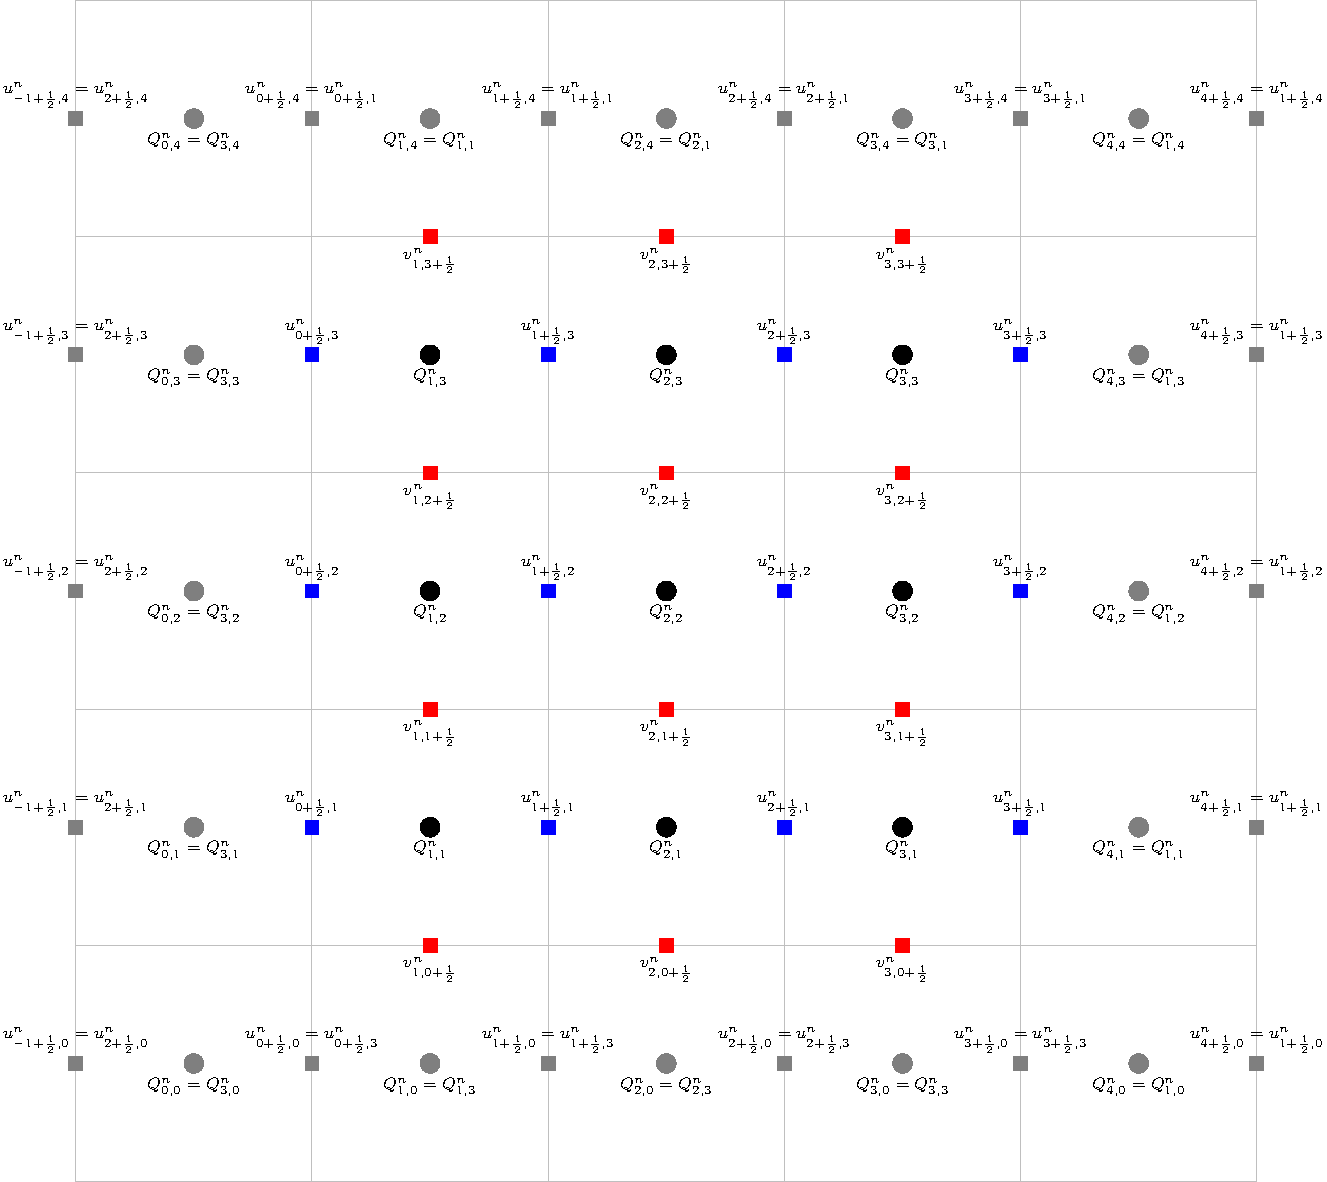
\includegraphics[width=1\linewidth]{2d_grid_function}
	\caption{Illustration of $(\Delta x, \Delta y)$-grid function $Q$ (black circles)
		and a $(\Delta x\Delta y)$-C grid wind $u$ (blue squares) and $v$ (red squares) and its ghost cell
		values (in gray) assuming biperiodicity.\label{chp3-sec1-grid2d-function}}
\end{figure}

We denote by $\nabla \cdot (q\boldsymbol{u})$ the divergence operator:
\begin{equation}
	\label{sec-adv2d:eqdiv}
	\nabla \cdot (q\boldsymbol{u})(x, y, t) =  
	[{\partial_x (uq)} + {\partial_y (vq)}](x, y, t).
\end{equation}
We recall that we say the $\boldsymbol{u}$ is \textbf{non-divergent} if $\nabla \cdot \boldsymbol{u}=0$.
We define the $(\Delta x, \Delta y)$-grid function $\delta^n$ as
the exact divergence of $q\boldsymbol{u}$ at the cell centers, namely
\begin{equation}
\label{2d-discrete-div}
\delta^n_{ij} = \nabla \cdot (\boldsymbol{u}q)(x_i,y_j,t^n).
\end{equation}
In this chapter, our focus also lies on periodic grid functions.
We define a $(\Delta x, \Delta y)$-grid function $Q$ as periodic if it satisfies the following conditions:
\begin{align*}
    Q_{i,j} &= Q_{N+i,j}, \quad i=-\nu+1, \ldots, 0,  \quad &j = -\nu+1, \ldots, M+\nu,\\
    Q_{i,j} &= Q_{i-N,j}, \quad i=N+1, \ldots, N+\nu, \quad &j = -\nu+1, \ldots, M+\nu,\\
    Q_{i,j} &= Q_{i,M+j}, \quad j=-\nu+1, \ldots, 0,  \quad &i = -\nu+1, \ldots, N+\nu,\\
    Q_{i,j} &= Q_{i,j-M}, \quad j=M+1, \ldots, M+\nu, \quad &i = -\nu+1, \ldots, N+\nu.
\end{align*}
We use the notation $\mathbb{P}^{N \times M}_{\nu}$ represent the spaces of periodic $(\Delta x, \Delta y)$-grid functions.
Similarly, we define a $(\Delta x, \Delta y)$-grid wind $(u,v)$ as periodic if it meets the following requirements:
\begin{align*}
    u_{i-\frac{1}{2},j} &= u_{N+i+\frac{1}{2},j} , \quad i=-\nu, \ldots, -1,   \quad &j = -\nu+1, \ldots, M+\nu,\\
    u_{i+\frac{1}{2},j} &= u_{i+\frac{1}{2}-N,j} , \quad i=N+1, \ldots, N+\nu, \quad &j = -\nu+1, \ldots, M+\nu,\\
    u_{i+\frac{1}{2},j} &= u_{i+\frac{1}{2},M+j} , \quad i=-\nu, \ldots, N+1+\nu,   \quad &j = -\nu+1, \ldots, 0,\\
    u_{i+\frac{1}{2},j} &= u_{i+\frac{1}{2},j-M} , \quad i=-\nu, \ldots, N+1+\nu,   \quad &j = M+1, \ldots, M+\nu,\\
    v_{i,j-\frac{1}{2}} &= v_{i,M+j+\frac{1}{2}} , \quad j=-\nu, \ldots, -1,   \quad &i = -\nu+1, \ldots, N+\nu,\\
    v_{i,j+\frac{1}{2}} &= v_{i,j+\frac{1}{2}-M} , \quad j=M+1, \ldots, M+\nu, \quad &i = -\nu+1, \ldots, N+\nu,\\
    v_{i,j+\frac{1}{2}} &= v_{N+i,j+\frac{1}{2}} , \quad j=-\nu, \ldots, M+1+\nu,   \quad &i = -\nu+1, \ldots, 0,\\
    v_{i,j+\frac{1}{2}} &= c_{i-N,j+\frac{1}{2}} , \quad j=-\nu, \ldots, N+1+\nu,   \quad &i = N+1, \ldots, N+\nu.\\
\end{align*}
In this case, we use the notation $u \in \mathbb{P}^{(N+1) \times M}_{\nu}$, 
$v \in \mathbb{P}^{N \times (M+1)}_{\nu}$.

For a grid function $Q$ we also use the notations:
\begin{align*}
Q_{\times,j} &:= (Q_{-\nu+1,j}, \ldots, Q_{N+\nu,j}) \in \mathbb{R}^N_{\nu},\\
Q_{i,\times} &:= (Q_{i,-\nu+1}, \ldots, Q_{i,M+\nu}) \in \mathbb{R}^M_{\nu}.
\end{align*}
Given $Q = (Q_{ij})\in \mathbb{P}^{N \times M}_{\nu, P}$, we define the $p$-norm by
\begin{equation}
	\label{chp3-pnorm}
	\|Q\|_{p,\Delta x \times \Delta y}=
	\begin{cases}
		\bigg( \sum_{i=1}^{N} \sum_{j=1}^{M}|Q_{ij}|^p \bigg)^{\frac{1}{p}} & \text{if } 1\leq p < \infty,\\
		\max_{i=1, \ldots, N,j=1,\ldots,M}{|Q_{ij}|} & \text{otherwise }.
	\end{cases}
\end{equation}
We also introduce the centered difference notation:
\begin{align}
	\label{sec-adv2d:eq6}
	\delta_x {h}(x_i,y, t) = 
	{h}(x_{i+\frac{1}{2}}, y, t) - 
	{h}(x_{i-\frac{1}{2}}, y, t), \\
	\delta_y {h}(x, y_j,t) = 
    {h}(x, y_{j+\frac{1}{2}},t) - 
    {h}(x, y_{j-\frac{1}{2}},t),
\end{align}
for any function $h: \Omega \times [0,T] \to \mathbb{R}$.
Additionally, we introduce the average value of $q$ in the control volume
$\Omega_{ij}$ at time $t$, denoted as ${Q}_{ij}(t)$, defined by:
\begin{equation}
	\label{chp3-sec1-not2}
	{Q}_{ij}(t) = \frac{1}{\Delta x \Delta y}
	\int_{x_{i-\frac{1}{2}}}^{x_{i+\frac{1}{2}}} \int_{y_{j-\frac{1}{2}}}^{y_{j-\frac{1}{2}}} {q}(x,y,t) \,dx.
\end{equation}
Moreover, we define the $(\Delta x, \Delta y)$-grid function of average values as $Q(t) = (Q_{ij}(t))_{i=-\nu+1,\ldots,N+\nu}^{j=-\nu+1,\ldots,M+\nu}$.

For the consideration of periodic boundary conditions, we can define spaces of periodic functions over 
the interval $\Omega$ as follows:
\begin{align*}
	\mathcal{S}_P(\Omega) &= \{q:\mathbb{R}^2\times[0,+\infty[\to \mathbb{R}: q(x+b-a,y+d-c,t)=q(x,y,t), \quad \forall x,y \in \mathbb{R}, \quad t\geq0\}.
\end{align*}
Similarly, the space of $k$-times periodically differentiable functions $\mathcal{C}_P^k(\Omega)$ can be defined as:
\begin{align*}
	\mathcal{C}_P^k(\Omega) &= \mathcal{S}_P(\Omega) \cap \mathcal{C}^k(\mathbb{R}^2\times[0,\infty[),
\end{align*}
where $\mathcal{C}^k(\mathbb{R}^2\times[0,+\infty[)$ denotes the space of functions that are $k$ 
times continuously differentiable in both the spatial and temporal variables.
In summary, $\mathcal{S}_P(\Omega)$ represents the space of periodic functions, and $\mathcal{C}_P^k(\Omega)$
represents the space of $k$-times periodically differentiable functions over $\Omega$ subject to periodic boundary conditions.

\subsection{The 2D advection equation}
Let us consider a  velocity field given by $\boldsymbol{u}=(u,v)$, where
$u$ is the velocity in $x$-direction and $v$ is the velocity in $x$ and $y$ direction
and $u,v \in \mathcal{C}^1_P(\Omega)$.
The two-dimensional advection equation in its differential form in 
a domain $\Omega$ associated to the velocity field $\boldsymbol{u}$ 
and assuming biperiodic boundary conditions is given by:
\begin{equation}
	\label{sec-adv2d:eq1}
	\begin{cases}
		[{\partial_t q} + {\partial_x (uq)} +  {\partial_y (vq)}](x, y, t)
		= 0, \quad \forall (x,y,t) \in \mathbb{R}^2\times ]0, +\infty[,\\
		{q}(a, y, t) = {q}(b, y, t), \quad \forall y \in [c,d],  \quad \forall t\geq 0, \\
		{q}(x, c, t) = {q}(x, d, t), \quad \forall x \in [a,b],  \quad \forall t\geq 0, \\
		q_0(x) = q(x,y,0), \quad \forall (x,y) \in \Omega.
	\end{cases}
\end{equation} 
A classical or strong solution to the two-dimensional advection equation is a 
$\mathcal{C}^1_P{(\Omega)}$ function ${q}$ satisfying Equation \eqref{sec-adv2d:eq1}.
As we did in Section \ref{chp2-sec1}, our goal is to deduce an
integral form of Equation \eqref{sec-adv2d:eq1}.
Thus, let us consider  $[x_1,x_2] \times [y_1, y_2]
\subset \Omega$ and $[t_1,t_2] \subset [0, +\infty[$.
Integrating Equation $\eqref{sec-adv2d:eq1}$ over 
$[x_1,x_2] \times [y_1, y_2]$ yields:
\begin{align}
	\label{sec-adv2d:eq2}
	\frac{d}{d t} \bigg(\int_{x_1}^{x_2} \int_{y_1}^{y_2}
	{q}(x, y, t) \,dx \,dy \bigg)=
	&-\int_{y_1}^{y_2} \bigg({(uq)}(x_2, y, t)
	-{(uq)}(x_1, y, t) \bigg) \,dy \\ \nonumber
	&-\int_{x_1}^{x_2} \bigg({(vq)}(x, y_2, t)
	-{(vq)}(x, y_1, t) \bigg) \,dx.
\end{align}
Integrating Equation \eqref{sec-adv2d:eq2} over the time interval $[t_1,t_2]$, 
we have:
\begin{align}
	\label{sec-adv2d:eq3}
	\int_{x_1}^{x_2} \int_{y_1}^{y_2}
	{q}(x, y, t_{n+1}) \,dx \,dy = &\int_{x_1}^{x_2} \int_{y_1}^{y_2}
	{q}(x, y, t_n) \,dx \,dy \\ \nonumber
	&-\int_{t_1}^{t_2} \int_{y_1}^{y_2} \bigg({(uq)}(x_2, y, t)
	-{(uq)}(x_1, y, t) \bigg) \,dy \,dt\\ \nonumber
	&-\int_{t_1}^{t_2} \int_{x_1}^{x_2} \bigg({(vq)}(x, y_2, t)
	-{(vq)}(x, y_1, t) \bigg) \,dx \,dt.
\end{align}
Equation \eqref{sec-adv2d:eq3} is the integral form of Equation 
\eqref{sec-adv2d:eq1}. We say that ${q}$ is a weak
solution to the advection equation \eqref{sec-adv2d:eq1} if ${q}$
satisfies the integral form \eqref{sec-adv2d:eq3}, 
$\forall [x_1,x_2]\times[y_1,y_2] \subset \Omega^{\mathrm{o}}$ and 
$\forall [t_1,t_2] \subset [0,+\infty[$.
We summarize the weak version of Equation \eqref{sec-adv2d:eq1} in Problem \eqref{chp3-sec2-prob1}.
\begin{prob}
	\label{chp3-sec2-prob1}
	Given an initial condition ${q}_0$ and
	a velocity function $\boldsymbol{u} = (u,v)$
 	we would like to find a weak solution ${q}$
	of the two-dimensional advection equation in its integral form:
	\begin{align*}
		\int_{x_1}^{x_2} \int_{y_1}^{y_2}
		{q}(x, y, t) \,dx \,dy = &\int_{x_1}^{x_2} \int_{y_1}^{y_2}
		{q}(x, y, t) \,dx \,dy \\ \nonumber
		&-\int_{t_1}^{t_2} \int_{y_1}^{y_2} \bigg({(uq)}(x_2, y, t)
		-{(uq)}(x_1, y, t) \bigg) \,dy \,dt\\ \nonumber
		&-\int_{t_1}^{t_2} \int_{x_1}^{x_2} \bigg({(vq)}(x, y_2, t)
		-{(vq)}(x, y_1, t) \bigg) \,dx \,dt.
	\end{align*}
	$\forall [x_1, x_2]\times [y_1, y_2] \times[t_1, t_2] \subset \Omega \times[0,T]$, 
	and ${q}(x, y, 0) = {q}_0(x, y)$, $\forall (x, y) \in \Omega$,
   ${q}(a, y, t) = {q}(b, y, t), \quad \forall y \in [c,d],  \quad \forall t\geq 0,$
   ${q}(x, c, t) = {q}(x, d, t), \quad \forall x \in [a,b],  \quad \forall t\geq 0.$
\end{prob}
Similarly to Section \ref{chp2-sec1}, Equation \eqref{sec-adv2d:eq1} and Problem \eqref{chp3-sec2-prob1} are equivalent
when ${q}, \boldsymbol{u} \in \mathcal{C}^1_P{(\Omega)}$.
For Problem \ref{chp3-sec2-prob1}, the total mass in $\Omega$ is defined by: 
\begin{equation}
	{M}_{\Omega}(t) = \int_{\Omega} {q}(x,y,t) \,dx \,dy , \quad \forall t \in [0,T],
\end{equation}
and is conserved within time: 
\begin{equation}
	{M}_{\Omega}(t) = {M}_{\Omega}(0), \quad \forall t \in [0,T].
\end{equation}
Considering a $(\Delta x, \Delta y, \Delta t, \lambda)$ discretization of $D = \Omega \times [0,T]$ and
substituting $t_1, t_2, x_1, x_2, y_1$ and $y_2$ by 
$t_{n}, t_{n+1}, x_{i-\frac{1}{2}}, x_{i+\frac{1}{2}}, y_{j-\frac{1}{2}}, y_{j+\frac{1}{2}}$,
respectively, in Equation \eqref{sec-adv2d:eq3}, we obtain:
\begin{align}
	\label{sec-adv2d:eq5}
	{Q}_{ij}(t_{n+1})  = {Q}_{ij}(t_{n})
	&- \frac{\Delta t}{\Delta x \Delta y}
	\delta _x \bigg( \frac{1}{\Delta t}
	\int_{t_1}^{t_2} \int_{y_{j-\frac{1}{2}}}^{y_{j+\frac{1}{2}}} 
	{(uq)}(x_{i}, y, t)
	\,dy \,dt \bigg) \\ \nonumber
	&- \frac{\Delta t}{\Delta x \Delta y}
	\delta _y \bigg( \frac{1}{\Delta t}
	\int_{t_1}^{t_2} \int_{x_{i-\frac{1}{2}}}^{x_{i+\frac{1}{2}}} 
	{(vq)}(x, y_{j}, t)
	\,dx \,dt \bigg),
\end{align}
where we are using the centered finite-difference notation.
Now we can define a discretized version of Problem \ref{chp3-sec2-prob1} as Problem \ref{chp3-sec2-prob2}.
\begin{prob}
	\label{chp3-sec2-prob2}
	Assume the framework of Problem \ref{chp3-sec2-prob1}
	and consider a $(\Delta x, \Delta y, \Delta t, \lambda)$-discretization of $\Omega\times [0,T]$.
	Since we are in the framework of Problem \ref{chp3-sec2-prob1}, it follows that:
	\begin{align*}
		{Q}_{ij}(t_{n+1})  = {Q}_{ij}(t_{n})
		&- {\lambda}
		\delta _x \bigg( \frac{1}{\Delta t \Delta y}
		\int_{t^n}^{t^{n+1}} \int_{y_{j-\frac{1}{2}}}^{y_{j+\frac{1}{2}}} 
		{(uq)}(x_{i}, y, t)
		\,dy \,dt \bigg) \\ \nonumber
		&- {\lambda}
		\delta _y \bigg( \frac{1}{\Delta t \Delta x}
		\int_{t^n}^{t^{n+1}} \int_{x_{i-\frac{1}{2}}}^{x_{i+\frac{1}{2}}} 
		{(vq)}(x, y_{j}, t)
		\,dx \,dt \bigg),
	\end{align*}
	where ${Q}_{ij}(t) = \frac{1}{\Delta x \Delta y}
	\int_{x_{i-\frac{1}{2}}}^{x_{i+\frac{1}{2}}} 
	\int_{y_{j-\frac{1}{2}}}^{y_{j+\frac{1}{2}}} {q}(x,y,t) \,dx \,dy$.
	Our problem now consists of finding the values ${Q}_{ij}(t_{n})$, 
	$\forall i = 1, \ldots, N$, $\forall j = 1, \ldots, M$, $\forall n = 0, \ldots, N_T-1$,
    given the initial values ${Q}_{ij}(0)$, $\forall i = 1, \ldots N$, $\forall j = 1, \ldots, M$.
    In other words, we aim to find the average values of ${q}$ in each control volume $\Omega_{ij}$ at the specified time instances.
\end{prob}
It is important to note that no approximations have been made in Problems \eqref{chp3-sec2-prob1} and \eqref{chp3-sec2-prob2}. 

\section{The finite-volume approach}
\label{sec:fv-2d}
Finally, we define the 2D-FV scheme problem as follows in Problem \ref{chp3-sec2-prob3}.
\begin{prob}[2D-FV scheme]
	\label{chp3-sec2-prob3}
	Assume the framework defined in Problem \ref{chp3-sec2-prob2}.
	The finite-volume approach of Problem \ref{chp3-sec2-prob1}
	consists of a finding a scheme of the form:
	\begin{align}
		\label{chp3-2dfv}
		{Q}_{ij}^{n+1} =  {Q}_{ij}^{n} - {\lambda} \delta_i {F}_{ij}^{n} - {\lambda} \delta_j {G}_{ij}^{n},
		\\ \nonumber \quad \forall i = 1, \ldots, N, \quad \forall j = 1, \ldots, M,
		\quad \forall n = 0, \ldots, N_T-1,
	\end{align}
	where $ \delta_i F_{ij}^n =
    {F}_{i+\frac{1}{2},j}^{n} 
    - {F}_{i-\frac{1}{2},j}^{n}$,
    $ \delta_j G_{ij}^n =
    {G}_{i,j+\frac{1}{2}}^{n} 
    - {G}_{i,j-\frac{1}{2}}^{n}$ 
    and ${Q}^{n}\in \mathbb{P}^{N\times M}_{\nu}$ is intended to be an approximation
	of ${Q}(t_{n})\in \mathbb{P}^{N\times M}_{\nu}$ in some sense. We define ${Q}_{ij}^{0} = {Q}_{ij}(0)$ or
	${Q}_{ij}^{0} = {q}^0_{ij}$.
    
    The term ${F}_{i+\frac{1}{2}, j}^{n}$ is known as numerical flux in the 
    $x$ direction and it approximates
	$\frac{1}{\Delta t \Delta y}\int_{t_n}^{t_{n+1}} 
    \int_{y_{j-\frac{1}{2}}}^{y_{j+\frac{1}{2}}} 
    (uq)(x_{i+\frac{1}{2}}, y, t) \,dy \,dt $,
    $\forall i = 0, 1, \ldots, N$, and 
	${G}_{i, j+\frac{1}{2}}^{n}$ is known as numerical flux in the 
    $y$ direction and it approximates
	$\frac{1}{\Delta t \Delta x}\int_{t_n}^{t_{n+1}}  
    \int_{x_{i-\frac{1}{2}}}^{x_{i+\frac{1}{2}}}
    (vq)(x, y_{j+\frac{1}{2}}, t) \,dx \,dt $,
    $\forall j = 0, 1, \ldots, M$,
	or, in other words, they estimate the time-averaged
    fluxes at the control volume $\Omega_{ij}$ boundaries.
\end{prob}
\begin{remark}
For Problem \ref{chp3-sec2-prob3}, we define the CFL number in the $x$ and $y$ direction
by $\max \{{|u_{i+\frac{1}{2},j}^n}|\}\frac{\Delta t}{\Delta x}$ and 
$\max \{ {|v_{i,j+\frac{1}{2}}^n}|\}\frac{\Delta t}{\Delta y}$, respectively.
The CFL number is maximum between these numbers and we say that the CFL condition is
satisfied if the CFL number is less than one. 
\end{remark}
For a 2D-FV the discrete total mass at the time-step $n$ is given by
\begin{equation*}
	M^n =  \Delta x \Delta y \sum_{i=1}^N \sum_{j=1}^M Q_{ij}^n.
\end{equation*}
Therefore, the discrete total mass is constant for a 2D-FV scheme,
which follows from a straightforward computation:
\begin{align*}
	M^{n+1} &=  \Delta x \sum_{i=1}^N  \sum_{j=1}^M Q_{ij}^{n+1} 
	= M^{n} - \Delta t  \sum_{i=1}^N  \sum_{j=1}^M (F^n_{i+\frac{1}{2},j}- F^n_{i-\frac{1}{2},j})
	 		 - \Delta t  \sum_{i=1}^N  \sum_{j=1}^M (G^n_{i,j+\frac{1}{2}}- G^n_{i,j-\frac{1}{2}})\\
	&= M^{n} - \Delta t \sum_{j=1}^M (F^n_{N+\frac{1}{2},j}- F^n_{\frac{1}{2},j})
			 - \Delta t \sum_{i=1}^N (G^n_{i,M+\frac{1}{2}}- G^n_{i,\frac{1}{2}})
	= M^{n},
\end{align*}
where we are using that $F^n_{N+\frac{1}{2},j} = F^n_{\frac{1}{2},j}$,
$G^n_{i,M+\frac{1}{2}} = G^n_{i,\frac{1}{2}}$ since we are assuming bi-periodic boundary
conditions.

As we mentioned in Problem \ref{chp3-sec2-prob3}, the initial condition may be assumed as $q_{ij}^0$ or $Q_{ij}(0)$. 
For two-dimensional simulations, we are going to assume  $q_{ij}^0$ as initial data to avoid the computation of integrals.
Furthermore, the errors will be calculated using the values $q_{ij}^n$ instead of $Q_{ij}(t_n)$.
Similarly to Proposition \ref{prop-bound-centroid}, we have that the centroid value approximates the average value
with second order, as Proposition \ref{prop-bound-centroid-2d} shows.
\begin{prop}
	\label{prop-bound-centroid-2d}
	If $q \in \mathcal{C}^2$, then $|Q_{ij}(t^n)-q_{ij}^n| \leq C_1 \Delta x^2 + C_2 \Delta x \Delta y + C_3 \Delta y^2$, where 
	$C_1$, $C_2$ and $C_3$ are constants.
\end{prop}
\begin{proof}
	Just apply Theorem \ref{prop-bound-midpoint2d} for the function $q(x,y,t^n)$.	
\end{proof}

In order to check the consistency of 2D-FV, it is useful to use the notion of discrete divergence.
\begin{definition}[Discrete divergence]
	\label{chp3-def-div}
	For Problem \ref{chp3-sec2-prob3}, we define the discrete divergence as a 
    $(\Delta x, \Delta y)$-grid function $\mathbb{D}^n(Q^n,u^n,v^n) \in \mathbb{P}^{N\times M}_{\nu}$
	given by:
	\begin{equation}
		\label{chp3-def-div-eq}
		\mathbb{D}_{ij}^n(Q^n,u^n,v^n)=  \frac{1}{\Delta t}
        \bigg(\frac{\delta_i {F}_{ij}^{n}}{\Delta x} + \frac{\delta_j {G}_{ij}^{n}}{\Delta y} \bigg), 
        \quad i = 1, \ldots, N, \quad j=1, \ldots,M.
	\end{equation}
\end{definition}
With the aid of the discrete divergence, we may rewrite Equation \eqref{chp3-2dfv} as:
\begin{align}
    \label{chp3-2dfv-div}
    {Q}^{n+1} =  {Q}^{n} - \Delta t \mathbb{D}^n(Q^n,u^n,v^n),
\end{align}
Notice that if we replace  $Q^n$ by the exact solution $Q(t^n)$ in Equation \eqref{chp3-2dfv-div}, we have
\begin{align}
    \label{chp3-div-tau}
    {Q}(t^{n+1}) =  {Q}(t^{n}) - \Delta t \mathbb{D}^n(Q(t^n),u^n,v^n) - \Delta t \tau^n,
\end{align}
where $\tau^n \in \mathbb{P}^{N\times M}_{\nu}$ is the local truncation error (LTE).
Rearranging the terms of Equation \eqref{chp3-div-tau}, we obtain:
\begin{align}
    \label{chp3-div-tau2}
    \tau^n =  \frac{{Q}(t^{n+1}) - {Q}(t^{n})}{\Delta t} - \mathbb{D}^n(Q(t^n),u^n,v^n).
\end{align}
We define the consistency of the 2D-FV scheme as follows.
\begin{definition}[Consistency]
	\label{chp3-def-cons}
	Let us consider the framework of Problem \ref{chp3-sec2-prob3}.
	A 2D-FV scheme is said to be consist in the $p$-norm if for any sequence of
	$(\Delta x^{(k)},\Delta y^{(k)}, \Delta t^{(k)},\lambda)$-discretizations, 
	$k \in \mathbb{N}$, with
    $\lim_{k\to \infty }{\Delta x^{(k)}} =\lim_{k\to \infty }{\Delta y^{(k)}}= \lim_{k\to \infty }{\Delta t^{(k)}} = 0$, we have:
	\begin{equation*}
		\lim_{k \to \infty}\bigg[ {\max_{1\leq n\leq N_T^{(k)}}}{\|\tau^n\|_{p,\Delta x^{(k)} \times \Delta y^{(k)}}} \bigg] = 0,
	\end{equation*}
	and it is said to be consistent with order $d$ in the $p-$norm if
	\begin{equation*}
		{\max_{1\leq n\leq N_T^{(k)}}}{\|\tau^n\|_{p,\Delta x^{(k)} \times \Delta y^{(k)}}} = O(\Delta x^d).
	\end{equation*}
\end{definition}
The relationship between consistency and convergence is explained in Section \ref{chp3-CCS}.
If $q$ satisfies Equation \eqref{sec-adv2d:eq1}, it can be observed that consistency is equivalent to the following:
\begin{equation*}
	{\max_{1\leq n\leq N_T^{(k)}}}{\|\delta^n - \mathbb{D}^n(Q^n,u^n,v^n)\|_{p,\Delta x^{(k)} \times \Delta y^{(k)}}} = O(\Delta x^d),
\end{equation*}
where $\delta^n \in \mathbb{P}^{N\times M}_{\nu}$ is defined in Equation \eqref{2d-discrete-div}.
Therefore, we can determine whether a 2D-FV scheme is consistent by comparing the discrete divergence to the exact divergence.

\section{Dimension splitting}
\label{sec-dsplit}
This section aims to demonstrate how a 2D-FV scheme, such as the one presented in Problem \ref{chp3-sec2-prob3},
can be constructed using 1D-FV schemes through a technique known as dimension splitting.
Before introducing the dimension splitting scheme proposed by \citet{lin:1996},
it is helpful to examine general operator splitting schemes,
as the dimension splitting technique is a specific instance of operator splitting methods.

For a given time interval $[0,T]$, we utilize a $\Delta t$-temporal grid. Let us consider the abstract Cauchy problem.
\begin{align*}
	\begin{cases}
		\frac{dq}{dt}(t) &= Aq(t), \quad t \in [t^n,t^{n+1}],\\
		q(t^n) &= q_n,
	\end{cases}
\end{align*}
for $n=0,\ldots, N_T-1$, where $q(t) \in \mathcal{B}$ for some Banach space $\mathcal{B}$, and $A:\mathcal{B} \to \mathcal{B}$ is a linear operator
following the framework of \citet[Chapter~3]{richtmyer:1968}.
We are interested in finding $q(t^{n+1})$ given $q_n$.
Assuming that $A = A_1 + A_2$ for two linear operators $A_1, A_2:\mathcal{B} \to \mathcal{B}$, we consider the following abstract Cauchy sub-problems:
\begin{align*}
	\begin{cases}
		\frac{dq^1}{dt}(t) &= A_1q(t), \quad t \in [t^{n},t^{n+1}],\\
		q^{1}(t^n) &= q_n,
	\end{cases}
\end{align*}
and
\begin{align*}
	\begin{cases}
		\frac{dq^{21}}{dt}(t) &= A_2q(t), \quad t \in [t^n,t^{n+1}],\\
		q^{21}(t^n) &= q^1(t^{n+1}).
	\end{cases}
\end{align*}
Then we can approximate $q(t_0 + \Delta t)$ as $q^{21}(t^n + \Delta t)$ 
with an error of $O(\Delta t)$ if $A_1$ and $A_2$ do not commute. 
Otherwise, this method is exact.
This approach is known as Lie-Trotter splitting. 
It's worth noting that the Lie-Trotter splitting can also be performed in reverse order when solving the sub-problems:
\begin{align*}
	\begin{cases}
		\frac{dq^2}{dt}(t) &= A_2q(t), \quad t \in [t^n,t^{n+1}],\\
		q^{2}(t^n) &= q_n,
	\end{cases}
\end{align*}
and 
\begin{align*}
	\begin{cases}
		\frac{dq^{21}}{dt}(t) &= A_1q(t), \quad t \in [t^n,t^{n+1}],\\
		q^{12}(t^n) &= q^1(t^{n+1}),
	\end{cases}
\end{align*}
and again we estimate $q(t^{n+1})$ by $q^{12}(t^{n+1})$ with error $O(\Delta t)$.
As noted by \citet{strang:1968}, we can consider the following equation 
to approximate $q(t^{n+1})$ using a second-order ($O(\Delta t^2)$) symmetric scheme:
\begin{equation}
	q^*(t^{n+1}) = \frac{q^{21}(t^{n+1}) + q^{12}(t^{n+1})}{2},
\end{equation}
This scheme is referred to as the average Lie-Trotter splitting \citep{holden:2010}.
The process of averaging two Lie-Trotter splittings is a specific case of methods
known as weighted sequential splitting methods in the literature.
Furthermore, this scheme averaging process can be extended to achieve higher-order schemes \citep{jia:2011}.
For an analysis of the accuracy of weighted sequential splitting methods, we recommend referring to \citet{csomos:2005}.

It is worth noting that one of the most commonly used second-order splitting schemes in the literature is the Strang splitting
\citep{strang:1968}.
This scheme requires solving three sub-problems per time-step, with one of them at time $t_n + \frac{\Delta t}{2}$.
In contrast, the average Lie-Trotter splitting requires solving four sub-problems per time-step.
Consequently, the Strang splitting is computationally more efficient.
However, as we will observe in this chapter, when applied to the linear advection equation, 
the average Lie-Trotter splitting allows for a modification that eliminates a splitting error
arising from considering a constant scalar field and non-divergent velocity \citep{lin:1996}.

To move towards the scheme from \citet{lin:1996}, let us consider Problem \ref{chp3-sec2-prob1} in its differential form (Equation \eqref{sec-adv2d:eq1}).
We are going to consider $N+2\nu$ one-dimensional advection equations in the $x$-direction:
\begin{equation*}
	\label{chp3-adv2deq-xdir1}
	[{\partial_t q^x}+{\partial_x (uq^x)}](x, y_j, t)
	= 0,
\end{equation*}
and the $N+2\nu$ one-dimensional advection equations in the $y$-direction
\begin{equation*}
	\label{chp3-adv2deq-ydir1}
	[{\partial_t q^y} +{\partial_y (vq^y)}](x_i, y, t) = 0.   
\end{equation*}
We shall assume that these problems are solved using a 1D-FV scheme as in Problem \ref{chp2-sec2-prob4}
with numerical flux functions ${F}_{i+\frac{1}{2},j}^n(Q^n_{\times,j},\tilde{u}^n_{i+\frac{1}{2},j})$ and
${G}^n_{i,j+\frac{1}{2}}(Q^n_{i,\times},\tilde{v}^n_{i,j+\frac{1}{2}})$, respectively
where $\tilde{u}^n_{i+\frac{1}{2},j}$ is the time-averaged used in the departure point estimation in the $x$ direction
and $\tilde{v}^n_{i,j+\frac{1}{2}})$ is the time-averaged used in the departure point estimation in the $y$ direction.
In this work, we assume that the fluxes ${F}_{i+\frac{1}{2},j}^n(Q^n_{\times,j},\tilde{u}^n_{i+\frac{1}{2},j})$ and
${G}^n_{i,j+\frac{1}{2}}(Q^n_{i,\times} ,\tilde{v}^n_{i,j+\frac{1}{2}})$ are computed using the PPM flux
assuming that the CFL number is less than one (see Equation \eqref{chp-sec-flux:numerical-flux3}).

More explicitly, as in Section \ref{chp2-sec-ppm}, 
we have a piecewise-parabolic approximation in the $x$ direction:
\begin{align}
	\label{chp3-ppmx-eq1}
	\begin{cases}
    q_{ij}^x(x;Q_{\times, j}^n) = q_{L,i,j}^x + \Delta q_{ij}^x z_i(x) + q_{6, i,j}^xz_i(x)(1-z_i(x)), \\
	z_i(x) = \frac{x-x_{i-\frac{1}{2}}}{\Delta x},
	\quad x \in X_i,\\
    q_{L, i,j}^x = q_{i-\frac{i}{2},j}^n+ O(\Delta x^2),\\
    q_{R, i,j}^x = q_{i+\frac{i}{2},j}^n+ O(\Delta x^2),\\
	\Delta q_{ij}^x = q_{R, i,j}^x - q_{L, i,j}^x,\\
	q_{6,i,j}^x = 6\bigg(Q_{ij}^n - \frac{(q_{L,i,j}^x + q_{R,i,j}^x)}{2}\bigg),
	\end{cases}
\end{align}
for $i=1, \ldots, N$, $j=-\nu+1, \ldots, M + \nu$, and we also construct a piecewise-parabolic
approximation in the $y$ direction:
\begin{align}
	\label{chp3-ppmy-eq2}
	\begin{cases}
	q_{ij}^y(y;Q_{i,\times}^n) = q_{L,i,j}^y + \Delta q_{ij}^y z_j(y) + q_{6, i,j}^yz_j(y)(1-z_j(y)),\\ 
	z_j(y) = \frac{y-y_{j-\frac{1}{2}}}{\Delta y},
	\quad y \in Y_j,\\
    q_{L, i,j}^y = q_{i,j-\frac{1}{2}}^n+ O(\Delta y^2),\\
    q_{R, i,j}^y = q_{i,j+\frac{1}{2}}^n+ O(\Delta y^2),\\
	\Delta q_{ij}^y = q_{R, i,j}^y - q_{L, i,j}^y,\\
	q_{6,i,j}^y = 6\bigg(Q_{ij}^n - \frac{(q_{L,i,j}^y + q_{R,i,j}^y)}{2}\bigg),
    \end{cases}
\end{align}
for $i=-\nu+1, \ldots, N + \nu$, $j=1, \ldots, M$.
The values $q_{L,i,j}^x$, $q_{R,i,j}^x$, $q_{L,i,j}^y$, and $q_{R,i,j}^y$,
which approximate the values of $q$ at C-grid wind positions, are computed
using one of the schemes PPM-0, PPM-PL07, PPM-CW84, or PPM-L04, as described
in Sections \ref{chp2-sec-ppm} and \ref{chp2-sec-mono}.
These approximations are expected to be
second-order accurate because the given average values are computed on the
2D control volume $\Omega_{ij}$ instead of the 1D control volumes $X_i$ or $Y_j$.
Then, we may express the fluxes as in Equation \eqref{chp-sec-flux:numerical-flux3}, namely:
\begin{align}
	\label{chp3-flux-xdir}
	F_{i+\frac{1}{2},j}^n ({Q^n_{\times,j},\tilde{u}^n_{i+\frac{1}{2},j}})= \tilde{u}^{n}_{i+\frac{1}{2},j}\times
	\begin{cases}
	q_{R,i,j}^x +\frac{1}{2}(q_{6,i,j}^x - \Delta q_{ij}^x){\tilde{c}_{i+\frac{1}{2},j}^{x,n}}
    +\frac{1}{3}{q_{6,i,j}^x}(\tilde{c}_{i+\frac{1}{2},j}^{x,n})^2,
    \quad &\text{if} \quad \tilde{u}_{i+\frac{1}{2},j}^n>0,\\
	q_{L,i+1,j}^x - \frac{1}{2}(q_{6,i+1,j}^x + \Delta q_{i+1,j}^x){\tilde{c}_{i+\frac{1}{2},j}^{x,n}}
    -\frac{1}{3}{q_{6,i+1,j}^x}(\tilde{c}_{i+\frac{1}{2},j}^{x,n})^2,
    \quad &\text{if} \quad \tilde{u}_{i+\frac{1}{2},j}^n\leq0,\\
    \end{cases}
\end{align}
for $i=0, \ldots, N$, $j=-\nu+1, \ldots, M + \nu$, and 
\begin{align}
	\label{chp3-flux-ydir}
	G_{i,j+\frac{1}{2}}^n ({Q^n_{i,\times},\tilde{v}^n_{i,j+\frac{1}{2}}})= \tilde{v}^{n}_{i,j+\frac{1}{2}}\times
	\begin{cases}
	q_{R,i,j}^y +\frac{1}{2}(q_{6,i,j}^y - \Delta q_{ij}^y){\tilde{c}_{i,j+\frac{1}{2}}^{y,n}}
    +\frac{1}{3}{q_{6,i,j}^y}(\tilde{c}_{i,j+\frac{1}{2}}^{y,n})^2,
    \quad &\text{if} \quad \tilde{v}_{i+\frac{1}{2},j}^n>0,\\
	q_{L,i,j+1}^y - \frac{1}{2}(q_{6,i,j+1}^y + \Delta q_{i,j+1}^y){\tilde{c}_{i,j+\frac{1}{2}}^{y,n}}
    -\frac{1}{3}{q_{6,i,j+1}^y}(\tilde{c}_{i,j+\frac{1}{2}}^{y,n})^2,
    \quad &\text{if} \quad \tilde{v}_{i,j+\frac{1}{2}}^n\leq0,\\
    \end{cases}
\end{align}
for $i=-\nu+1, \ldots, N + \nu$, $j=0, \ldots, M$, and 
\begin{align*}
\tilde{c}_{i+\frac{1}{2},j}^{x,n} = \tilde{u}_{i+\frac{1}{2},j}^{x,n}\frac{\Delta t}{\Delta x},\\
\tilde{c}_{i,j+\frac{1}{2}}^{y,n} = \tilde{v}_{i,j+\frac{1}{2}}^{y,n}\frac{\Delta t}{\Delta y},
\end{align*}
are the time-averaged CFL numbers in the $x$ and $y$ directions, respectively,
which are assumed to have absolute value less than one.
The time-averaged winds are computed using the RK1 and RK2 schemes from Section \ref{chp2-sec-dp}.
When we use the PPM-L04 scheme, we set $\nu=4$; otherwise, $\nu=3$.

We introduce the auxiliary grid functions $\mathbf{F}$ and $\mathbf{G}$, both belonging to $\mathbb{R}^{N\times M}_{\nu}$, given by:
\begin{align*}
	\mathbf{F}_{ij}({Q^n,\tilde{u}^n}) = -\lambda \big({F}_{i+\frac{1}{2},j}^n(Q^n_{\times,j},\tilde{u}^n_{i+\frac{1}{2},j})-
                                                  {F}_{i-\frac{1}{2},j}^n(Q^n_{\times,j},\tilde{u}^n_{i-\frac{1}{2},j}) \big),
\end{align*}
for $i=1, \ldots, N$, $j=-\nu+1, \ldots, M + \nu$, and
\begin{align*}
	\mathbf{G}_{ij}({Q^n,\tilde{v}^n}) = -\lambda \big({G}_{i,j+\frac{1}{2}}^n(Q^n_{i,\times},\tilde{v}^n_{i,j+\frac{1}{2}})-
                                                  {G}_{i,j-\frac{1}{2}}^n(Q^n_{i,\times},\tilde{v}^n_{i,j-\frac{1}{2}}) \big),
\end{align*}
for $i=-\nu+1, \ldots, N + \nu$  $j=1, \ldots, $,
which are the numerical flux update of the 1D-FV schemes in the $x$ and $y$ direction, respectively.
The Lie-Trotter splitting is obtained by solving the advection in the $x$ direction
\begin{align*}
	{Q}^{x,n} =  {Q}^{n} + \mathbf{F}({Q^n}, \tilde{u}^n),
\end{align*}
for $j=\nu+1, \ldots, M+\nu$ (Figure \ref{lt-Qx}), and then we advect in the $y$ direction with initial data ${Q}^{x,n}$ 
\begin{align*}
	{Q}^{yx,n} = Q^{x,n} + \mathbf{G}({Q}^{x,n},\tilde{v}^n),
\end{align*}
for $i=-\nu+1, \ldots, N+\nu$ (Figure \ref{lt-FQx}).
To get the average Lie-Trotter splitting we repeat the process in the reverse order by solving the advection equation
in the $y$ direction
\begin{align*}
	{Q}^{y,n} =  {Q}^{n} + \mathbf{G}({Q^n},\tilde{v}^n),
\end{align*}
for $i=-\nu+1, \ldots, N+\nu$ (Figure \ref{lt-Qy}), and then we advect in the $x$-direction with initial data ${Q}^{y,n+1}$ 
\begin{align*}
	{Q}^{xy,n} = Q^{y,n} + \mathbf{F}(Q^{y,n},\tilde{u}^n),
\end{align*}
for $j=-\nu+1, \ldots, M+\nu$, (Figure \ref{lt-GQy}) and thus we have the average Lie-Trotter solution:
\begin{align*}
	Q^{n+1} &= \frac{(Q^{xy,n} + Q^{yx,n})}{2} \\
    &= Q^n + \frac{1}{2}\mathbf{F}(Q^n,\tilde{u}^n) + \frac{1}{2}\mathbf{G}(Q^n,\tilde{v}^n) + 
    \frac{1}{2}\mathbf{F}\bigg(Q^n + \mathbf{G}(Q^n, \tilde{v}^n), \tilde{u}^n\bigg)+
    \frac{1}{2}\mathbf{G}\bigg(Q^n + \mathbf{F}(Q^n, \tilde{u}^n), \tilde{v}^n\bigg),
\end{align*}
assuming that the numerical flux functions are linear in the input $Q$, we may rewrite a computationally cheaper version
of the average Lie-Trotter splitting as \citep{lin:1996}:
\begin{align}
	\label{chp3-avlt}
	Q^{n+1} =  Q^n+
	\mathbf{F}\bigg(Q^n + \frac{1}{2}\mathbf{G}(Q^n, \tilde{v}^n), \tilde{u}^n \bigg) +  
	\mathbf{G}\bigg(Q^n + \frac{1}{2}\mathbf{F}(Q^n, \tilde{u}^n), \tilde{v}^n \bigg).
\end{align}
\begin{figure}[!htb]
	\centering
	\begin{subfigure}{0.3\textwidth}
		\centering
		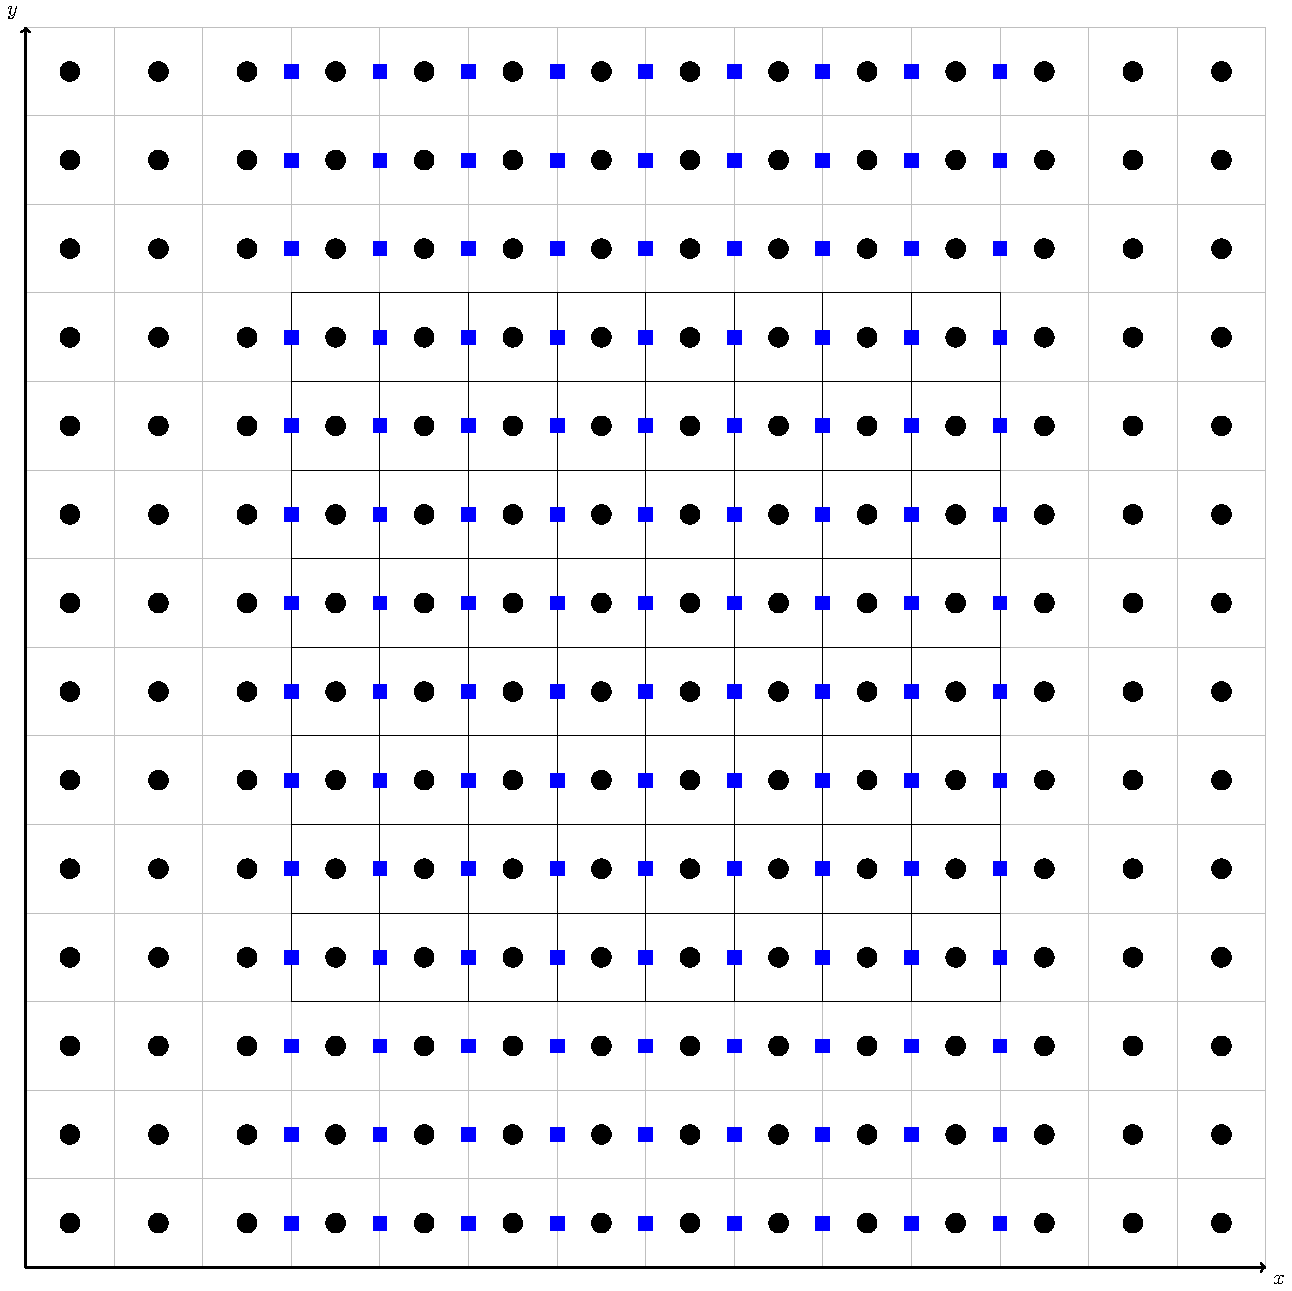
\includegraphics[width=1\linewidth]{2d_grid_Qx}
		\caption{$Q^n$ (black circles) and $u$ at edges (blue squares). \label{lt-Qx}}
	\end{subfigure}
	\begin{subfigure}{0.3\textwidth}
		\centering
		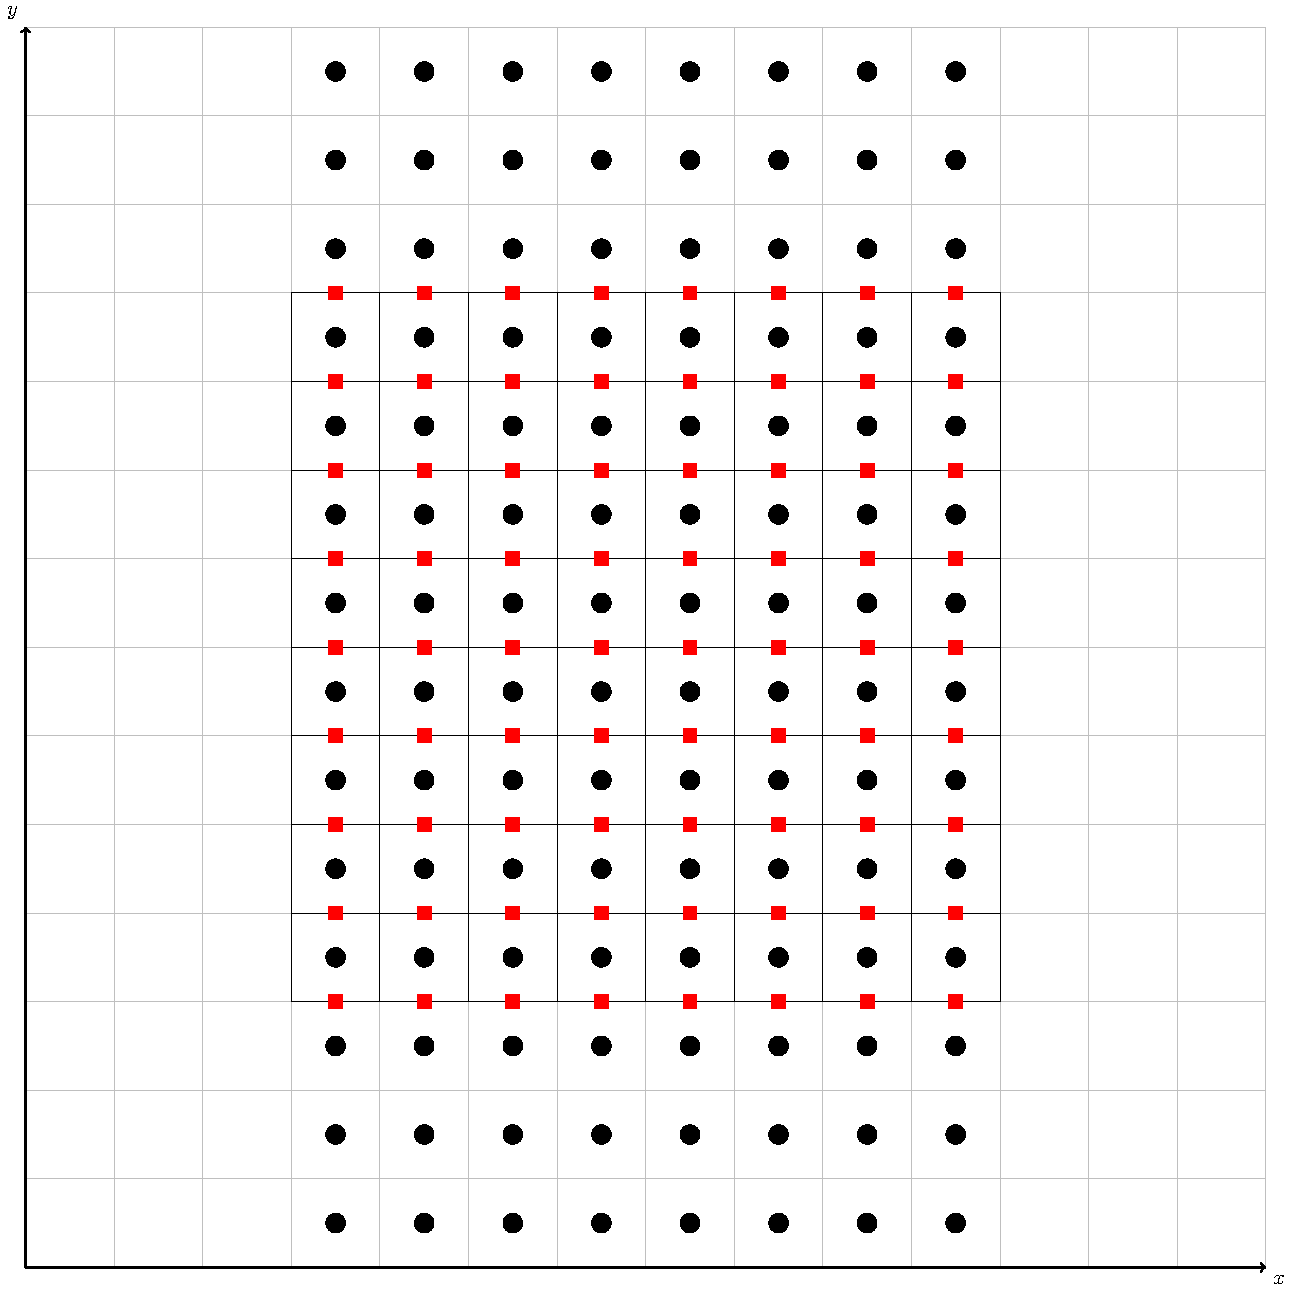
\includegraphics[width=1\linewidth]{2d_grid_FQ}
		\caption{$Q^{x,n}$ (black circles) and $v$ at edges (red squares).\label{lt-FQx} }
	\end{subfigure}
	\begin{subfigure}{0.3\textwidth}
	    \centering
	    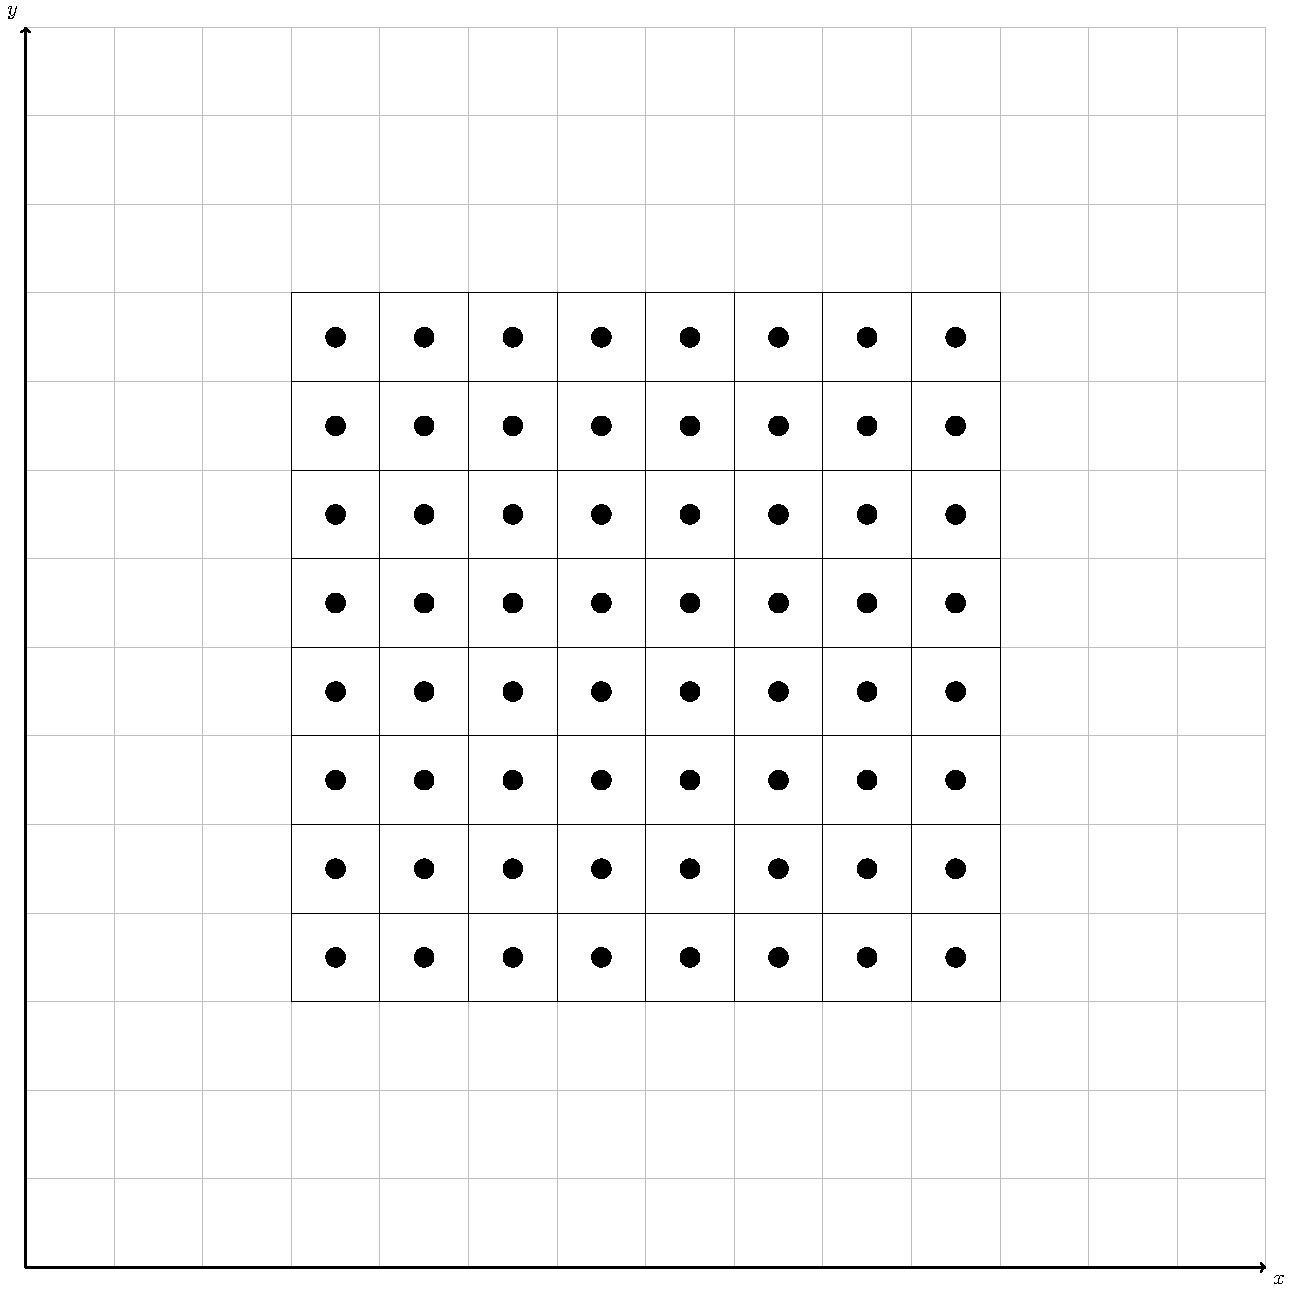
\includegraphics[width=1\linewidth]{2d_grid_GFQ}
		\caption{$Q^{yx,n}$ (black circles). \label{lt-GFQx}}
    \end{subfigure}
	\caption{Illustration of the Lie-Trotter splitting applied in the $x$ direction (operator $\mathbf{F}$)
	and then in the $y$ direction (operator $\mathbf{G}$). Interior cells are depicted using black lines,
	 while ghost cells are depicted using gray lines. 
	 All the winds shown are the ones used in the RK1 departure point scheme.
	 If the RK2 scheme is used, an additional layer of wind ghost values should be added at each boundary in (a) and (b). \label{ltxdir}}
\end{figure}

\begin{figure}[!htb]
	\centering
	\begin{subfigure}{0.3\textwidth}
		\centering
		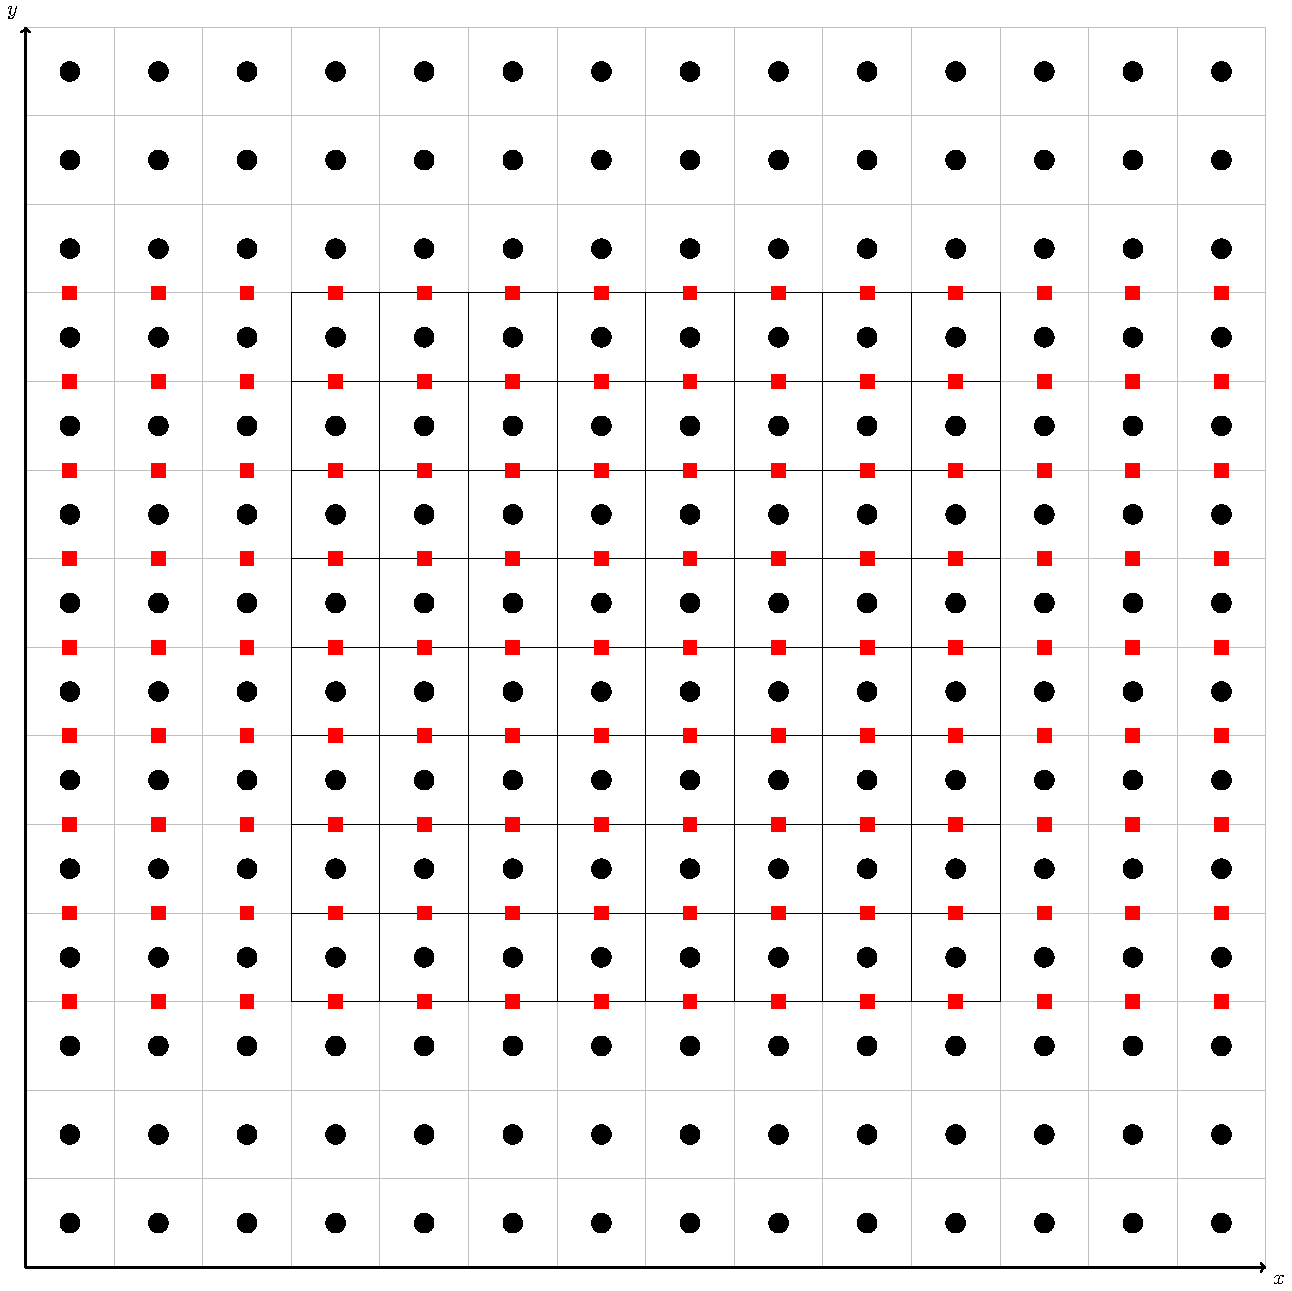
\includegraphics[width=1\linewidth]{2d_grid_Qy}
		\caption{$Q^n$ (black circles) and $v$ at edges (red squares). \label{lt-Qy}}
	\end{subfigure}
	\begin{subfigure}{0.3\textwidth}
		\centering
		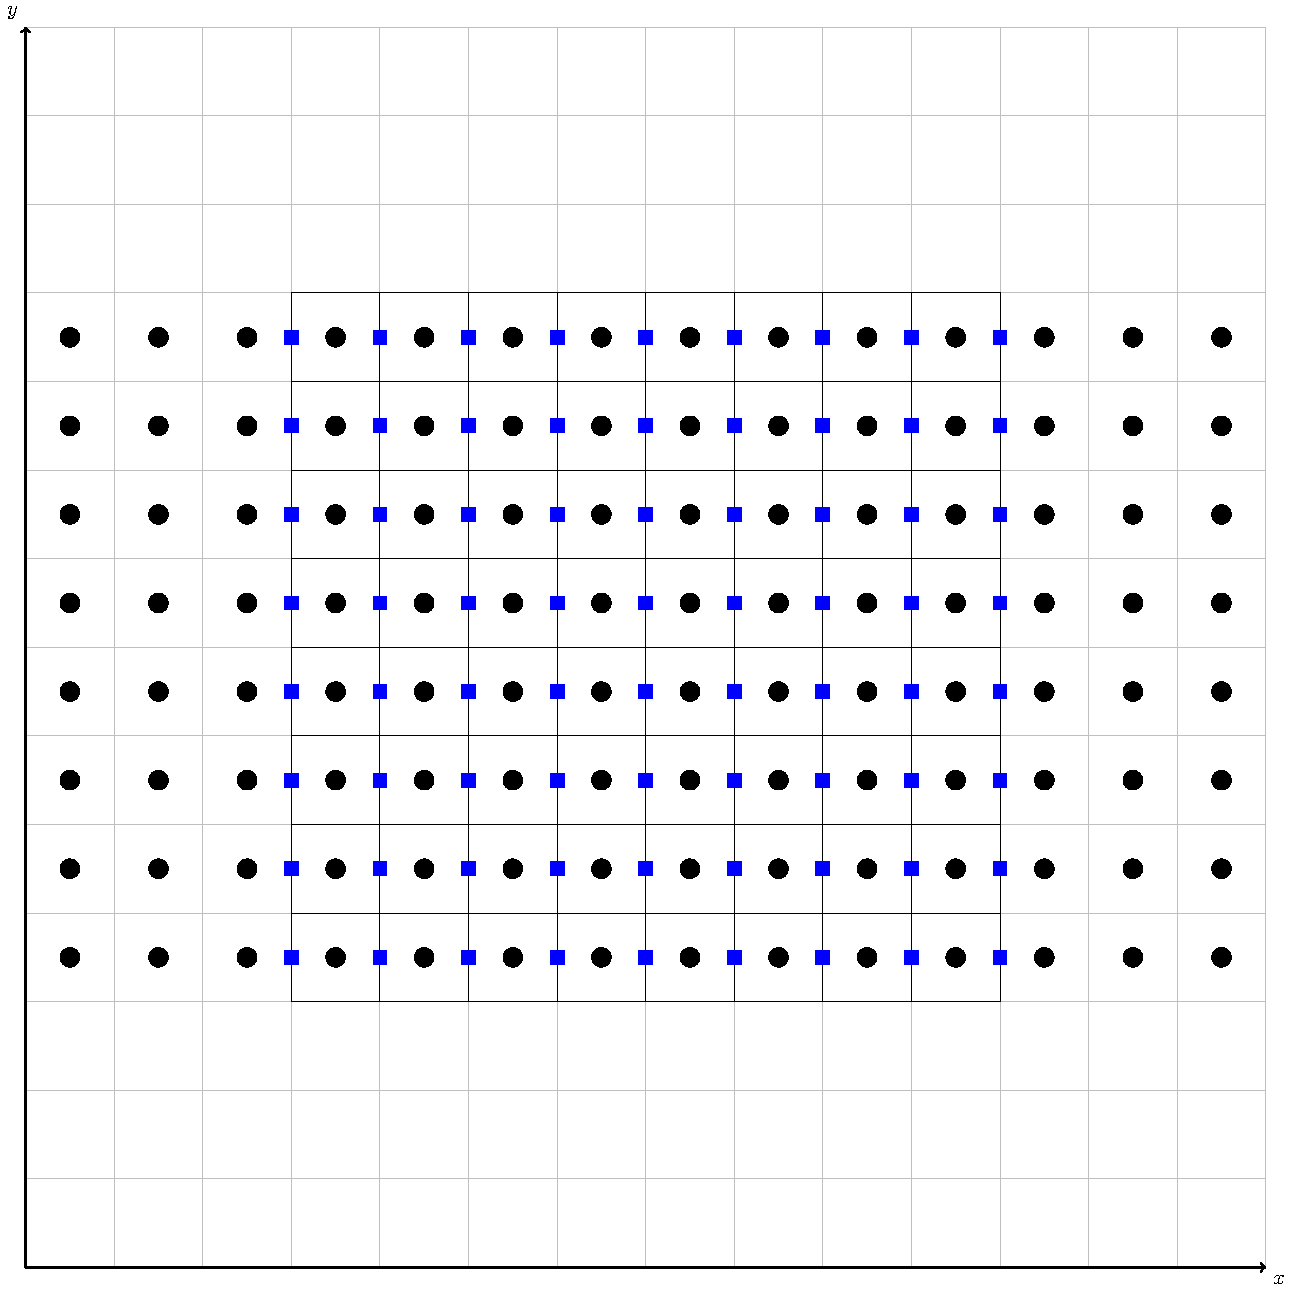
\includegraphics[width=1\linewidth]{2d_grid_GQ}
		\caption{$Q^{y,n}$ (black circles) and $u$ at edges (blue squares).\label{lt-GQy} }
	\end{subfigure}
	\begin{subfigure}{0.3\textwidth}
		\centering
		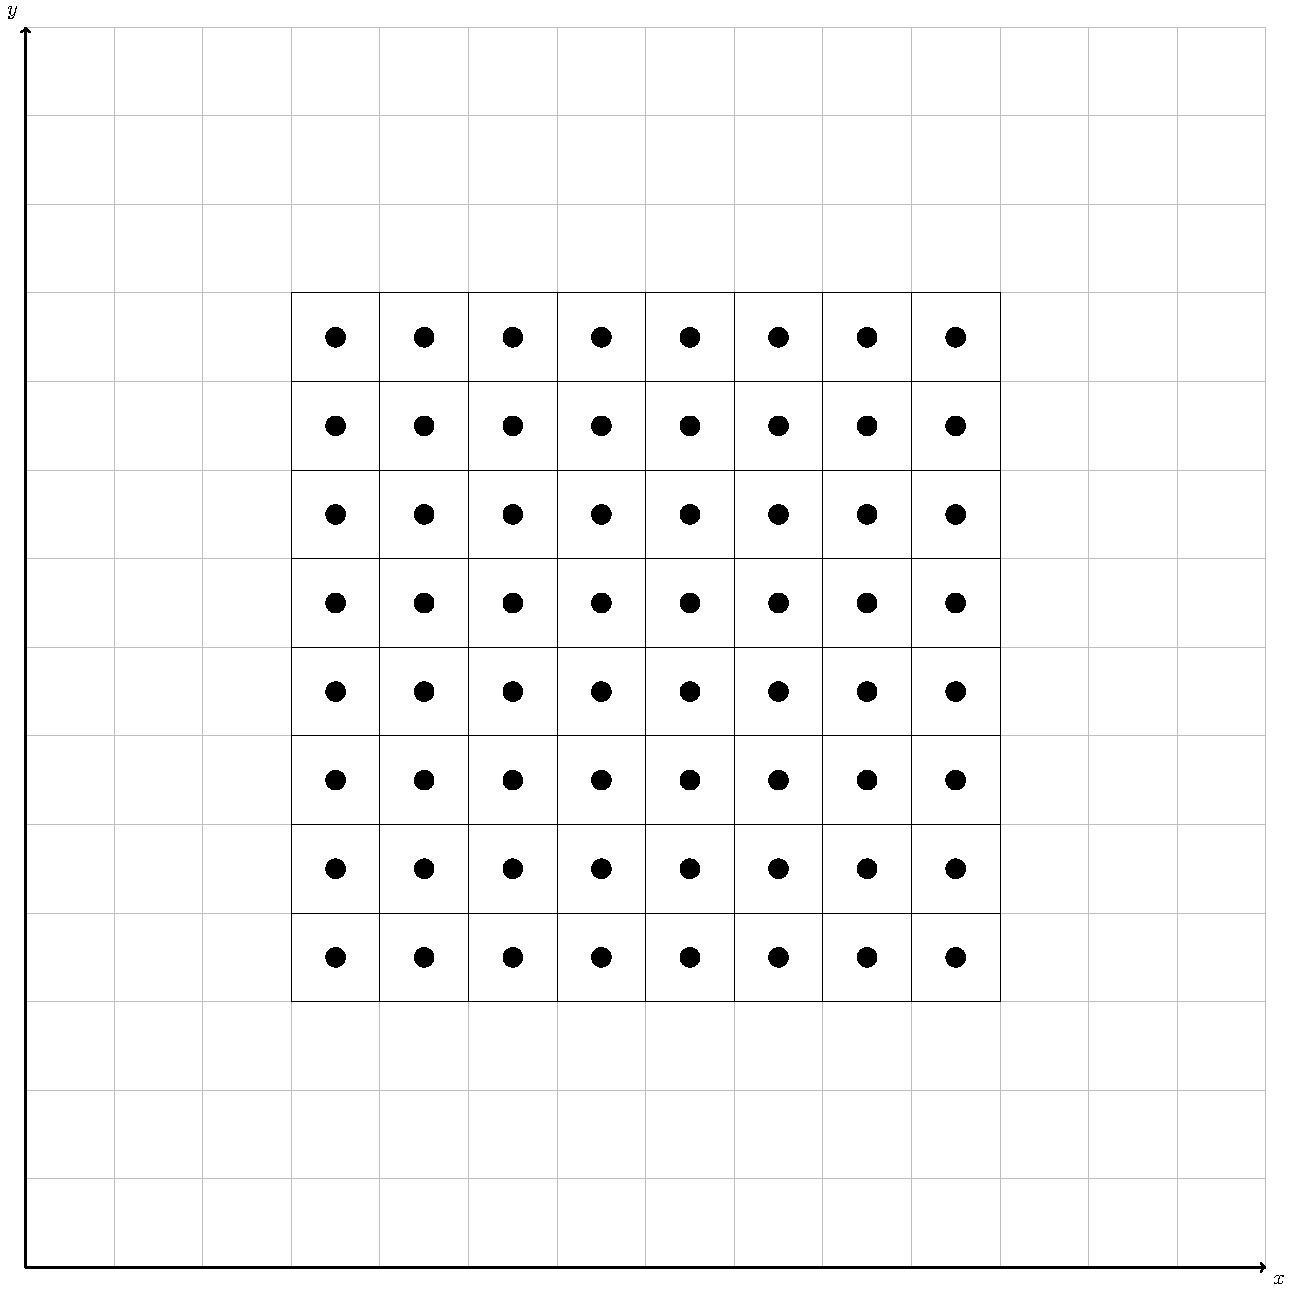
\includegraphics[width=1\linewidth]{2d_grid_GFQ}
		\caption{$Q^{xy,n}$ (black circles). \label{lt-FGQy}}
	\end{subfigure}
	\caption{Similar to Figure \ref{ltxdir} but considering the Lie-Trotter splitting in reverse order.}
\end{figure}
The numerical flux functions defined in Chapter \ref{chp-1d-fv} are indeed linear the 
input $Q$ if there are no monotonic constrain, but we are going to consider this scheme
even when there are monotonic constraints since it requires fewer operations.
Further, if we if assume that $q = \overline{q}$ is constant and $\nabla \cdot 
\boldsymbol{u} = 0$ then the solution remains constant and then, assuming also that
$\boldsymbol{u}$ does not depend on $t$, then $\mathbf{F}$ and $\mathbf{G}$ are given by
\begin{align*}
	\mathbf{F}_{ij}(Q^n,\tilde{u}^n) = -\overline{q} \lambda {\delta_x} u(x_i,y_j),\\
	\mathbf{G}_{ij}(Q^n,\tilde{v}^n) = -\overline{q} \lambda {\delta_y} v(x_i,y_j).
\end{align*}
However, if we compute the updated solution using Equation \eqref{chp3-avlt}, we have that the error is given by
\begin{align}
	\label{chp3-avlt-error}
	Q^{n+1}_{ij} - \overline{q} &= 
	-\Delta t \bigg(\frac{\delta_x u(x_i,y_j)}{\Delta x} + 	\frac{\delta_y v(x_i,y_j)}{\Delta y} \bigg)
	-\Delta t^2 \overline{q}\bigg( \frac{\delta_y v \delta_x u(x_i,y_j) + \delta_x u\delta_y v(x_i,y_j)}{2\Delta x \Delta y} \bigg) \\
	&= \Delta t (O(\Delta x^2) + O(\Delta y^2))
	   -\Delta t^2 \overline{q}\bigg( \frac{\delta_y v \delta_x u(x_i,y_j) + \delta_x u\delta_y v(x_i,y_j)}{2\Delta x \Delta y} \bigg).
\end{align}
Thus, the terms in the equation above multiplied by $\Delta t^2$ are related to an splitting error, even if we consider the exact fluxes.
Aiming to eliminate the error from, \citet{lin:1996} proposes to consider a modification of the average Lie-Trotter splitting as
\begin{align}
	\label{chp3-avlt2}
	Q^{n+1} = Q^n +  
	\mathbf{F}\bigg(Q^n + \frac{1}{2}\mathbf{g}(Q^n, \tilde{v}^n), \tilde{u}^n \bigg) +  
	\mathbf{G}\bigg(Q^n + \frac{1}{2}\mathbf{f}(Q^n, \tilde{u}^n), \tilde{v}^n \bigg),
\end{align}
where $\mathbf{f}$ and $\mathbf{g}$ are called inner advective operators and approximate
$-\Delta t u \frac{\partial q}{\partial x}$ and $-\Delta t v \frac{\partial q}{\partial y}$.

In this work, we shall consider the following inner advective operator proposed by
\citet{lin:2004} (hereafter, \textbf{L04}) and the one proposed by \citet{putman:2007} (hereafter, \textbf{PL07}).
The PL07 scheme is currently used in the FV3 dynamical core.
We also shall consider the average Lie-Trotter splitting (hereafter, \textbf{AVLT}). 
All the expressions of each inner advective operator mentioned are shown in Table \ref{chp3-tab1}.
It is easy to see that both operators {L04} and {PL07} eliminate the term multiplied by
$\Delta t^2$ that appeared in Equation \eqref{chp3-avlt-error} when we apply these operators for a 
constant grid function $Q^n$ and a non-divergent velocity field in Equation \eqref{chp3-avlt2}.
Therefore, these inner advective operators eliminate the splitting error for a constant field and a non-divergent velocity field.
\begin{table}[!h]
	\begin{tabular}{|c|l|l|}
		\hline
		Scheme & \multicolumn{1}{c|}{$\mathbf{f}_{ij}(Q^n, \tilde{u}^n)$} & \multicolumn{1}{c|}{$\mathbf{g}_{ij}(Q^n,\tilde{v}^n)$} \\ \hline
		AVLT   & $\mathbf{F}_{ij}(Q^n,\tilde{u}^n)$ 
		       & $\mathbf{G}_{ij}(Q^n,\tilde{v}^n)$ \\ \hline
		L04    & $\mathbf{F}_{ij}(Q^n,\tilde{u}^n) + Q_{ij}^n
				 \frac{\Delta t}{\Delta x}(\tilde{u}_{i+\frac{1}{2},j}^n - \tilde{u}_{i-\frac{1}{2},j}^n)$ 
		       & $\mathbf{G}_{ij}(Q^n, \tilde{v}^n) + Q_{ij}^n
				 \frac{\Delta t}{\Delta y}(\tilde{v}_{i,j+\frac{1}{2}}^n - \tilde{v}_{i,j-\frac{1}{2}}^n)$ \\ \hline
		PL07   & $\frac{1}{2}\bigg(-Q_{ij}^n +
		       \frac{Q_{ij}^n + \mathbf{F}_{ij}(Q^n,\tilde{u}^n)}{1 - \frac{\Delta t}{\Delta x}\big(\tilde{u}_{i+\frac{1}{2},j}^n - \tilde{u}_{i-\frac{1}{2},j}^n\big)} 
		       \bigg)$
			   & $\frac{1}{2}\bigg(-Q_{ij}^n +
			   \frac{Q_{ij}^n + \mathbf{G}_{ij}(Q^n,\tilde{v}^n)}{1 - \frac{\Delta t}{\Delta y}\big(\tilde{v}_{i,j+\frac{1}{2}}^n - \tilde{v}_{i,j-\frac{1}{2}}^n\big)}
			   \bigg)$
			   \\ \hline
	\end{tabular}
\caption{Expression of the inner advective operators considered in this work.
AVLT stands for the average Lie-Trotter scheme, while L04 and PL07 stands for the inner
advective operators from \citet{lin:2004} and from \citet{putman:2007}, respectively.}
\label{chp3-tab1}
\end{table}

Recalling the definition of discrete divergence (Definition \ref{chp3-def-div}) we have:
\begin{equation}
	\mathbb{D}^n = -\frac{1}{\Delta t}
	\bigg[
     \mathbf{F}\bigg(Q^n + \frac{1}{2}\mathbf{g}(Q^n,\tilde{v}^n), \tilde{u}^n \bigg) 
	+\mathbf{G}\bigg(Q^n + \frac{1}{2}\mathbf{f}(Q^n,\tilde{u}^n), \tilde{v}^n \bigg) \bigg],
\end{equation}
and as pointed out in Section \ref{chp3-CCS}, we may use the discrete divergence to check the scheme consistency. 

\section{Numerical experiments}
\label{sec-ds-exp}
To assess the dimension splitting schemes introduced previously, 
we are going to consider the linear advection equation on $[0,1]\times[0,1]$ 
with bi-biperiodic boundary conditions.
For the 1D schemes, we consider the FV-SL schemes PPM-0, PPM-PL07, PPM-CW84, PPM-L04
with the departure point schemes RK1 and RK2 as in Section \ref{chp2-sec-numerical-exp}.
For all simulations, the CFL number is set to $0.8$, and the time integration interval 
is $[0,5]$, which represents the period of the exact solution for all tests.
We employ $(\Delta x^{(k)},\Delta y^{(k)},\lambda)$-discretizations with $\Delta x^{(k)} = \Delta y^{(k)} = 1/2^k$,
$\Delta t^{(k)} = 0.05/2^{k-4}$ for $k=4, \ldots, 10$, and $\lambda = 0.8$.
We introduce the relative error in the maximum norm:
\begin{equation*}
	E_k = \max_{n=0,\ldots, N_T}
	\frac{\| Q^n - q(t^n) \|_{\infty, \Delta x \times \Delta y}}
	{\|q(t^n)\|_{\infty, \Delta x \times \Delta y}}.
\end{equation*}
The convergence rate is defined as in Section \ref{chp2-sec-numerical-exp}, 
as well as the total mass variation, which is preserved with machine precision
in all experiments presented here.
Notice that in the error computation, we use the centroid values instead
of the exact average values to avoid computations of analytical integrals.
As we pointed out in Proposition \ref{prop-bound-centroid-2d}, this approximation introduces a second-order error.
As a first test, we consider a constant velocity $\boldsymbol{u}=(0.2,-0.2)$.
We are going to consider as initial condition a rectangular profile
(Figure \ref{chp3-sec-exp-adv1-e}) given by:
\begin{equation}
	\label{chp3-ic1}
	q_0(x,y) =  
	\begin{cases}
		1 & \text{if } (x,y) \in [0.4,0.6]\times [0.4,0.6],\\
		0 & \text{otherwise}.
	\end{cases}
\end{equation}

\begin{figure}[!htb]
	\centering
	\begin{subfigure}{0.4\textwidth}
		\centering
		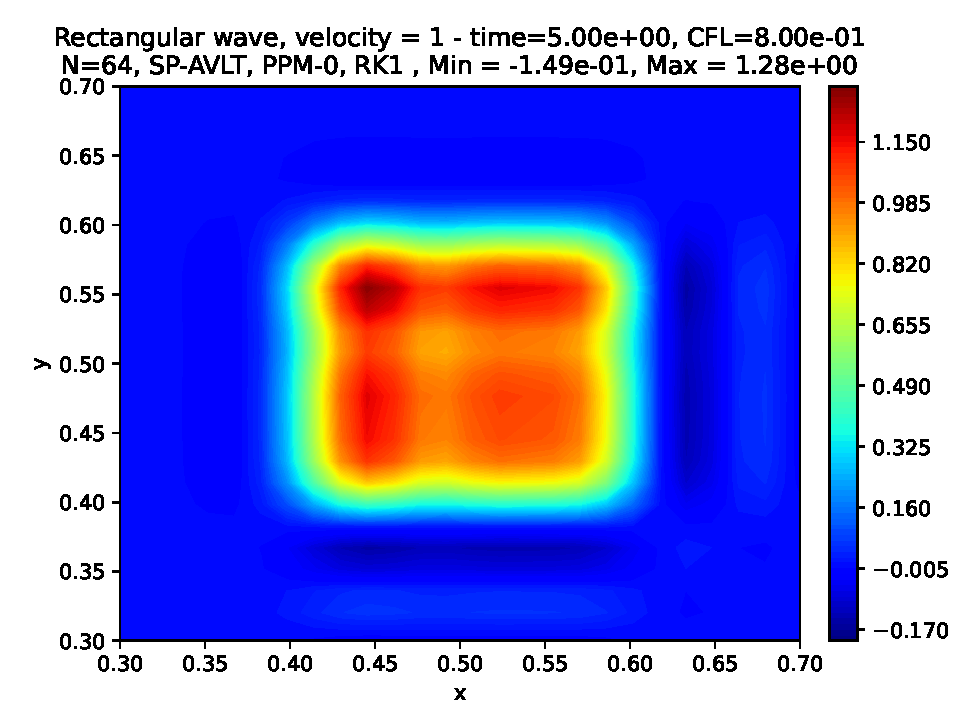
\includegraphics[width=1\linewidth]{2d_adv_tc1_ic3_vf1_t80_N64_SP-AVLT_PPM-0_RK1}
		\caption{PPM-0.\label{chp3-sec-exp-adv1-a}}
	\end{subfigure}
	\begin{subfigure}{0.4\textwidth}
		\centering
		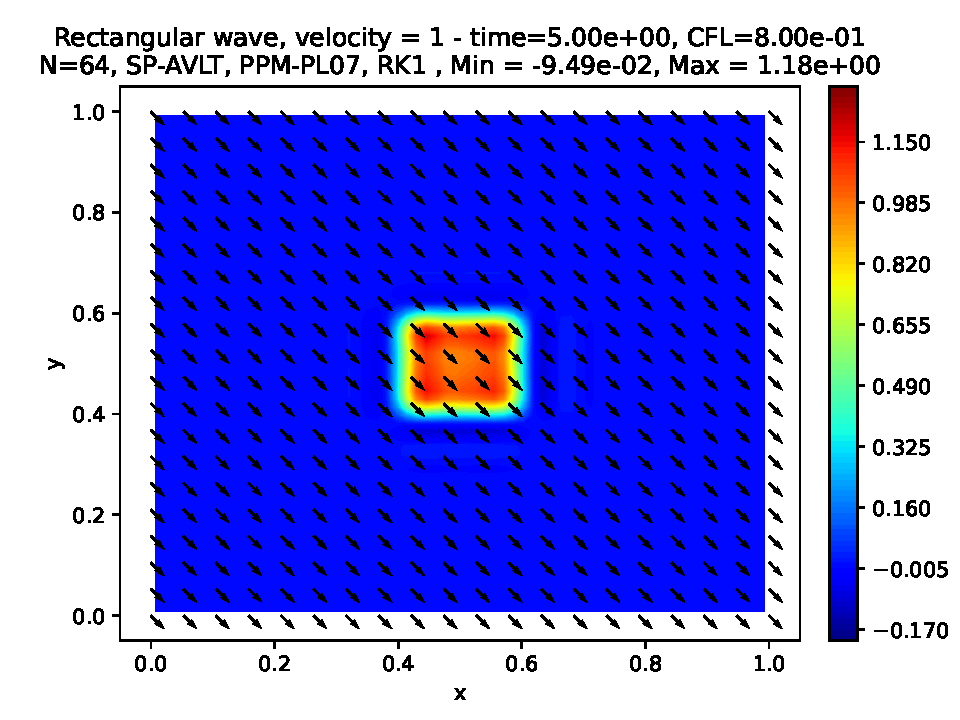
\includegraphics[width=1\linewidth]{2d_adv_tc1_ic3_vf1_t80_N64_SP-AVLT_PPM-PL07_RK1}
		\caption{PPM-PL07.\label{chp3-sec-exp-adv1-b}}
	\end{subfigure}
	
	\begin{subfigure}{0.4\textwidth}
		\centering
		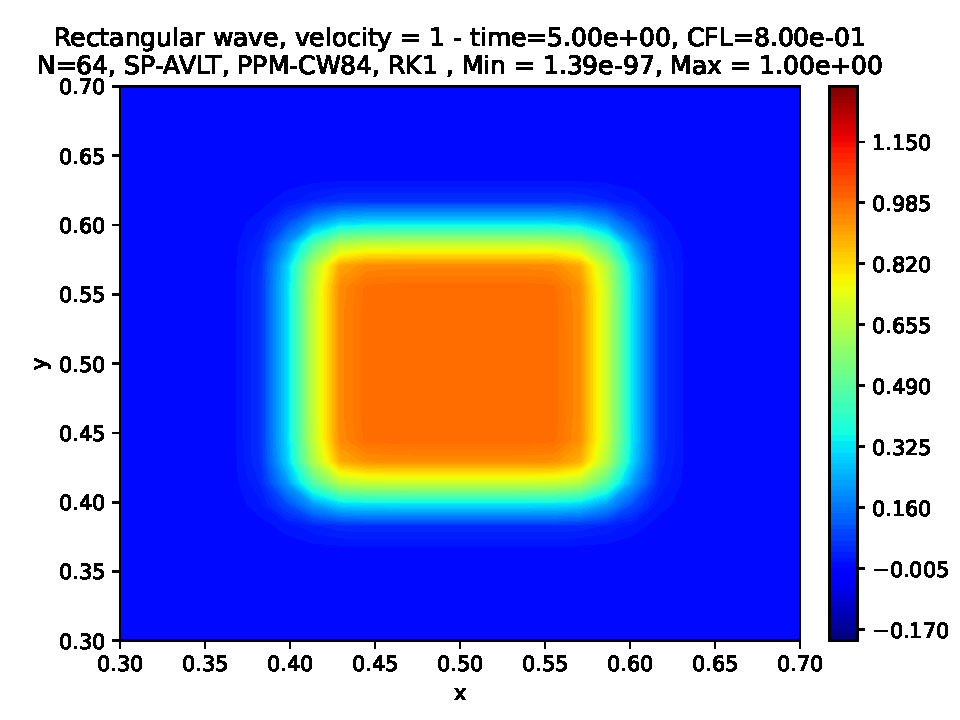
\includegraphics[width=1\linewidth]{2d_adv_tc1_ic3_vf1_t80_N64_SP-AVLT_PPM-CW84_RK1}
		\caption{PPM-CW84.\label{chp3-sec-exp-adv1-c}}
	\end{subfigure}
	\begin{subfigure}{0.4\textwidth}
		\centering
		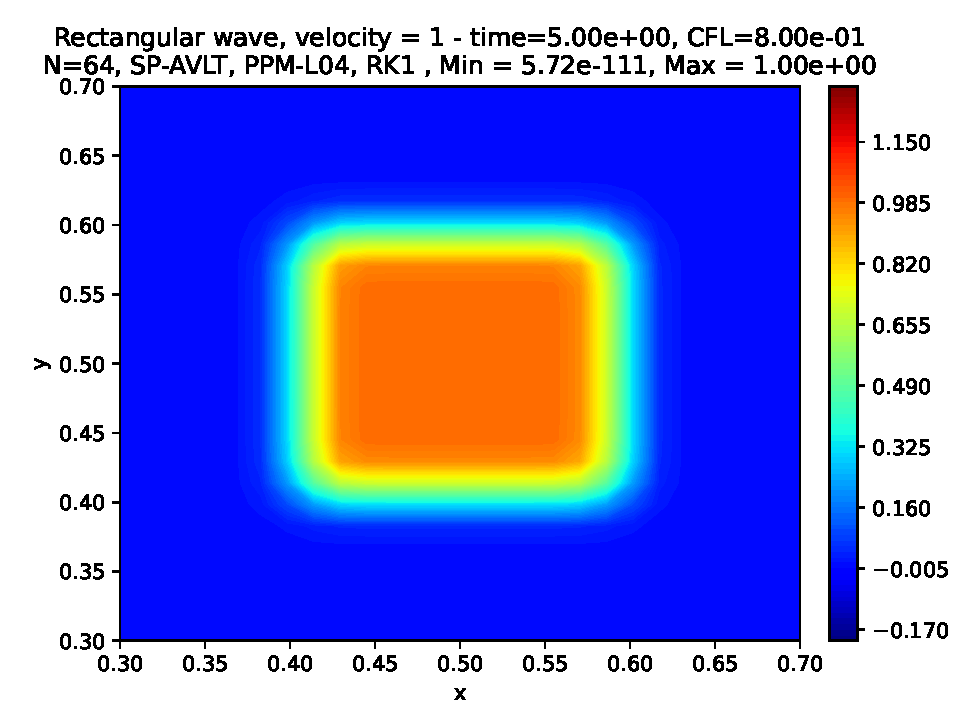
\includegraphics[width=1\linewidth]{2d_adv_tc1_ic3_vf1_t80_N64_SP-AVLT_PPM-L04_RK1}
		\caption{PPM-L04.\label{chp3-sec-exp-adv1-d}}
	\end{subfigure} 

	\begin{subfigure}{0.4\textwidth}
	\centering
	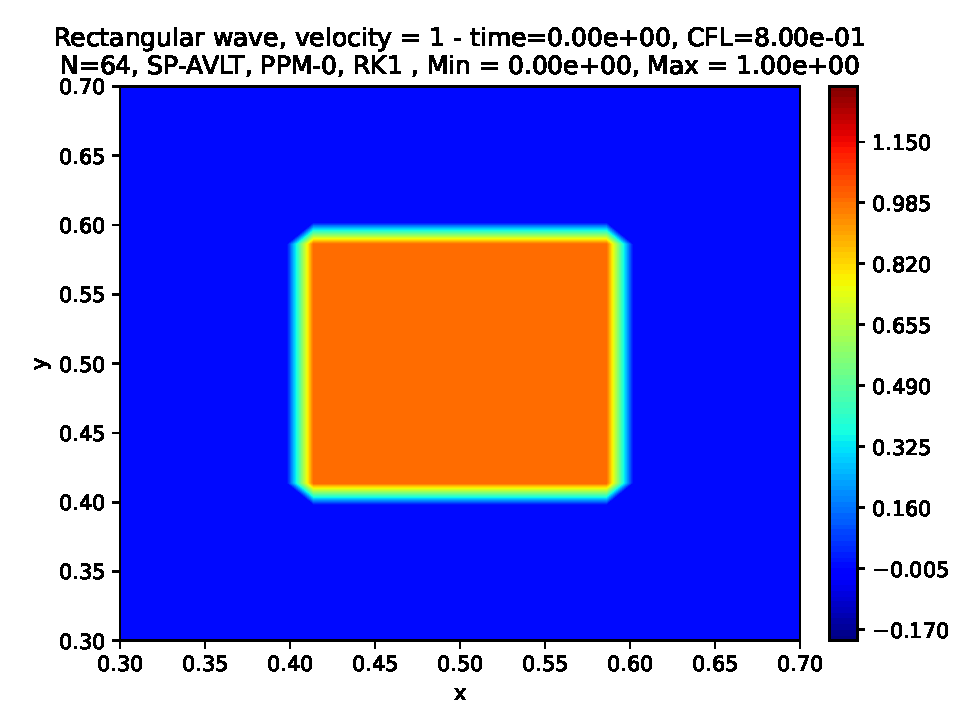
\includegraphics[width=1\linewidth]{2d_adv_tc1_ic3_vf1_t0_N64_SP-AVLT_PPM-0_RK1}
	\caption{Initial condition.\label{chp3-sec-exp-adv1-e}}
	\end{subfigure} 

	\caption{Linear advection experiment using a constant velocity equal to 
		$\boldsymbol{u} = (0.2,-0.2)$,
		a CFL number equal to $0.8$, $N=M=64$, and the initial condition is given by Equation \eqref{chp3-ic1}.
		We use the schemes PPM-0, PPM-PL07, PPM-CW84 and PPM-L04 with AVLT splitting.
		These figures show the advected profile after 5 time units (one time period).
		The initial condition is shown in (e).
		\label{chp3-sec-exp-adv1}}
\end{figure}

The exact solution of Problem \ref{chp3-sec2-prob1} in this case is 
$q_0((x,y)-\boldsymbol{u}t)$. Since the velocity field is constant, all the splitting 
schemes introduced in Section \ref{sec-dsplit} are 
the same, so we will only consider the AVLT splitting. 
Additionally, it can be easily seen that the Lie-Trotter splitting is exact in 
this case (cf. eg. \cite[p.~202-203]{leveque:1990}), meaning no splitting error is introduced.
For the 1D schemes, we use RK1 to compute 
the departure point since this scheme is exact when the velocity is constant.

The conclusions for this test are very similar to the first 1D test from Section \ref{chp2-sec-numerical-exp}.
This behavior is due to the fact that no splitting error is introduced when the velocity is constant.
From Figure \ref{chp3-sec-exp-adv1}, it can be observed that the AVLT splitting preserves monotonicity
when we use the monotonic 1D schemes PPM-CW84 and PPM-L04.
For the non-monotonic schemes, as seen in Figure \ref{chp2-sec-exp-adv1},
PPM-PL07 produces less numerical dispersion than PPM-0, similar to the first 1D test.

For variable velocity testing, we consider two Gaussian hills given by:
\begin{align}
	\begin{split}
	\label{chp3-ic2}
	q_0(x,y) = &\exp(-10\cos^2 (\pi (x-0.1))\exp(-10\cos^2 (\pi y)) + \\
			   &\exp(-10\cos^2 (\pi (x+0.1))) \exp(-10\cos^2 (\pi y)),
	\end{split}
\end{align}
defined in $[0,1] \times [0,1]$, whose graph is shown in Figure \ref{chp3-sec-exp-adv2-ic}.
\begin{figure}[!htb]
	\begin{subfigure}{0.45\textwidth}
		\centering
		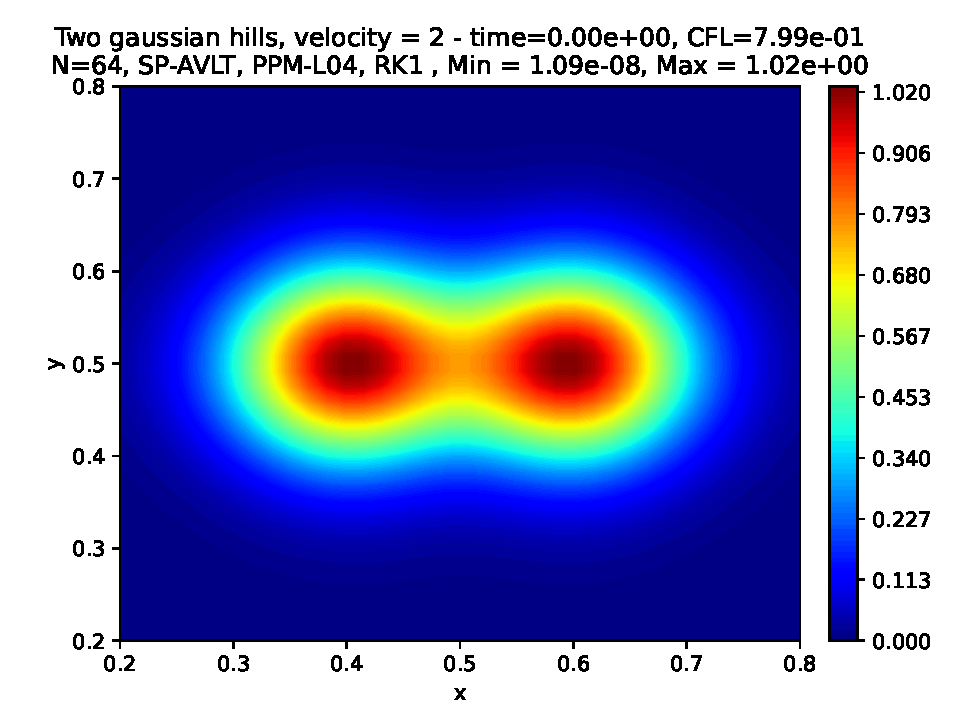
\includegraphics[width=1\linewidth]{2d_adv_tc1_ic4_vf2_t0_N64_SP-AVLT_PPM-L04_RK1}
		\caption{Initial condition from Equation \eqref{chp3-ic2}.\label{chp3-sec-exp-adv2-ic}}
	\end{subfigure} 
\end{figure}

We consider the Cartesian version of the deformational flow test case on the sphere from \citet{nair:2010}
proposed by \citet{chen:2017}. The velocity is given by:
\begin{equation}
	\label{chp3-vf1}
	\begin{cases}
		u(x,y,t) &= c\frac{\pi}{L_y}\sin^2(\alpha_1)(2\cos(\alpha_2)\sin(\alpha_2))(\cos(\alpha_3)) - \frac{L_x}{T},\\
		v(x,y,t) &= \frac{-c}{\pi}\frac{2\pi}{L_x}(2\sin(\alpha_1)\cos(\alpha_1)\cos^2(\alpha_2))\cos(\alpha_3),
	\end{cases}
\end{equation}
where $L_x = 2\pi$, $L_y = \pi$, $T=5$, $c = \frac{10}{T}(\frac{L_x}{2\pi})^2$, $\alpha_1 = 2\pi\big(\frac{X}{L_x}-\frac{t}{T}\big)$, $\alpha_2 = \frac{\pi Y}{L_y}$,
$\alpha_3 =\frac{\pi t}{T}$,  $X = -\pi + 2\pi x $, $Y =-\frac{\pi}{2} +\pi y$. 
\citet{chen:2017} uses periodic boundary conditions in the $x-$direction and zero-gradient in the $y-$direction.
However, we will employ biperiodic boundary conditions to simplify the problem.
Both velocity fields are divergence-free, and they deform the initial condition.
After 5 time units, the scalar field returns to its initial position and shape, allowing us to compute the error.

In Figure \ref{chp3-sec-exp-adv2}, the results obtained using two Gaussian hills and
the velocity field from Equation \eqref{chp3-vf1} are depicted.
The PPM-L04 scheme with AVLT, L04, and PL07 splitting, along with RK1 as 
the departure point scheme, is used.
It can be observed how the scalar field deforms and eventually returns to its initial position.
Comparing the schemes, it is noticeable that the PL07 and L04 schemes produce almost identical
results and are less diffusive than AVLT.

From Figure \ref{chp3-sec-exp-adv2-error1}, it can be observed that when using the RK1 schemes,
the PL07 and L04 schemes are slightly more accurate than AVLT for the 1D PPM-PL07 schemes.
All these schemes exhibit a convergence order greater than two (Figure \ref{chp3-sec-exp-adv2-cr}).
When the 1D scheme PPM-L04 is used, all the splitting methods yield very similar results, regardless
of the departure point scheme.
However, when the RK2 schemes are used, AVLT is the most accurate and achieves a
third-order convergence (Figure \ref{chp3-sec-exp-adv2-error2}).
\begin{figure}[!htb]
	\centering
	\begin{subfigure}{0.4\textwidth}
		\centering
		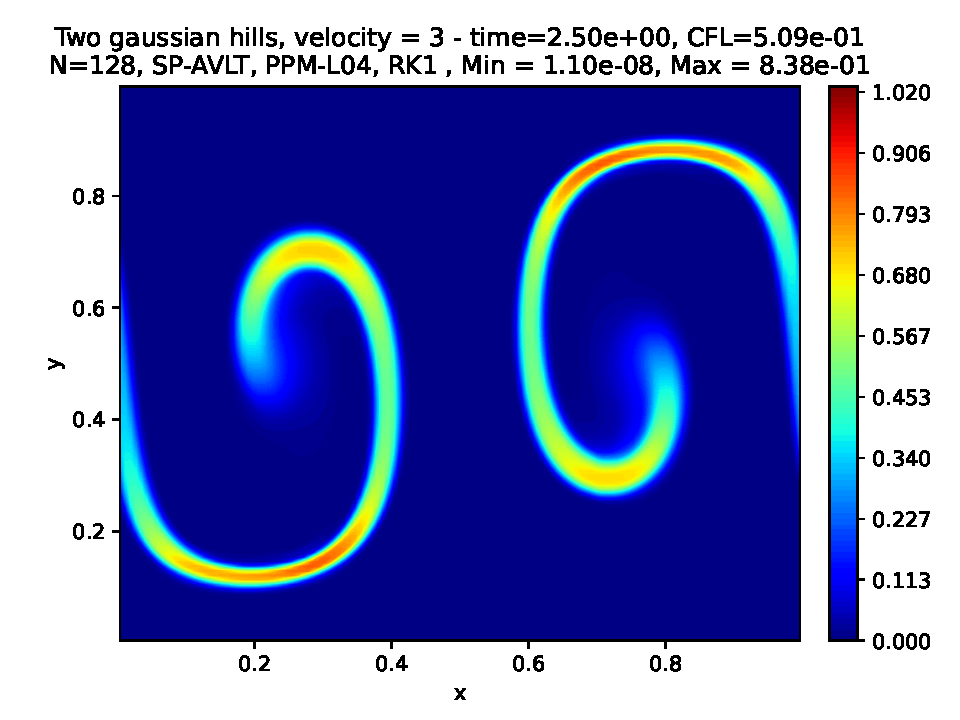
\includegraphics[width=1\linewidth]{2d_adv_tc1_ic4_vf3_t400_N128_SP-AVLT_PPM-L04_RK1}
		\caption{AVLT splitting at $t=2.5$.\label{chp3-sec-exp-adv2-a}}
	\end{subfigure}
	\begin{subfigure}{0.4\textwidth}
		\centering
		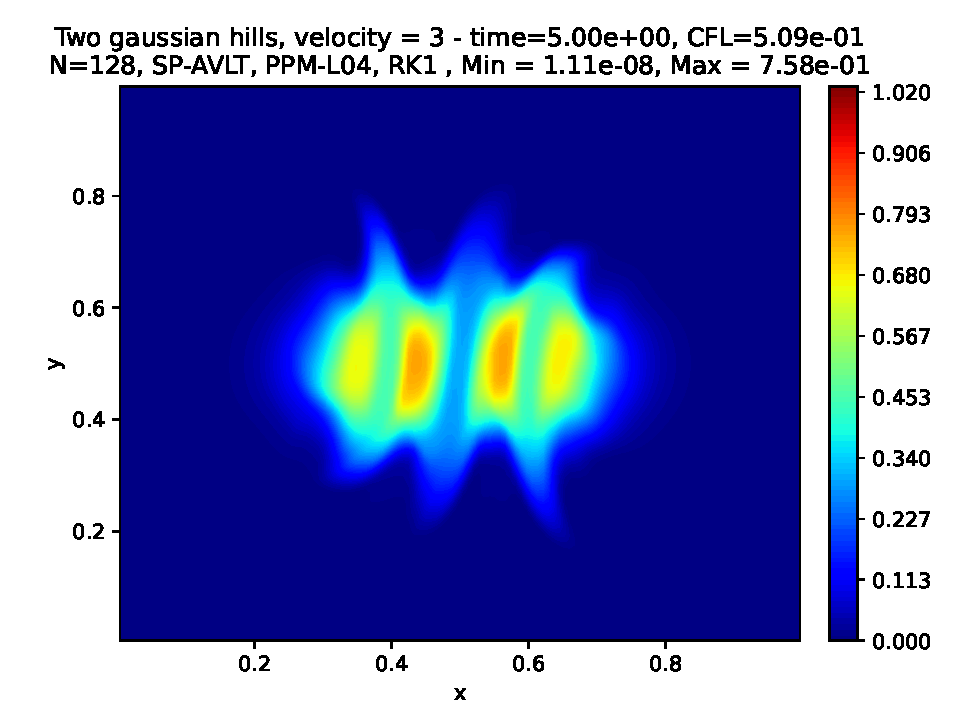
\includegraphics[width=1\linewidth]{2d_adv_tc1_ic4_vf3_t800_N128_SP-AVLT_PPM-L04_RK1}
		\caption{AVLT splitting at $t=5$.\label{chp3-sec-exp-adv2-b}}
	\end{subfigure}
	
	\begin{subfigure}{0.4\textwidth}
		\centering
		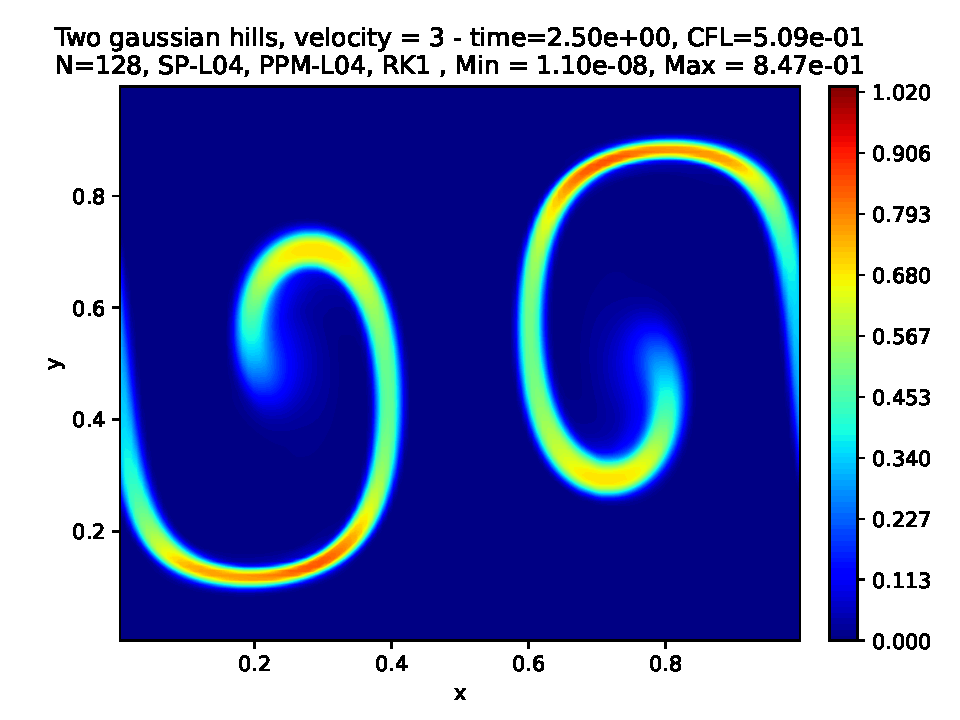
\includegraphics[width=1\linewidth]{2d_adv_tc1_ic4_vf3_t400_N128_SP-L04_PPM-L04_RK1}
		\caption{L04 splitting at $t=2.5$.\label{chp3-sec-exp-adv2-c}}
	\end{subfigure}
	\begin{subfigure}{0.4\textwidth}
		\centering
		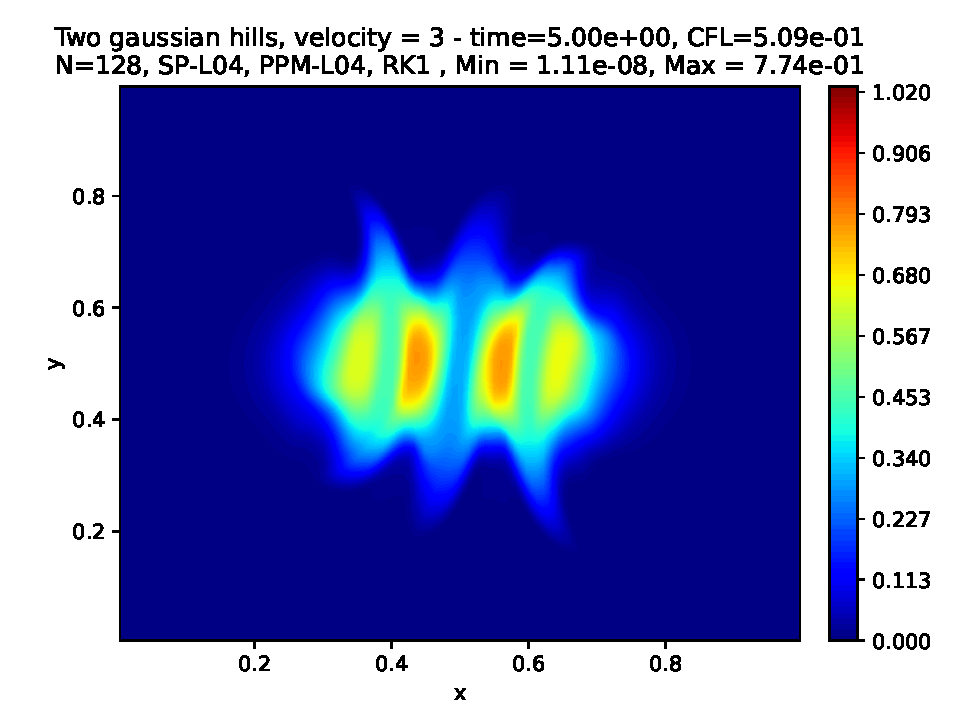
\includegraphics[width=1\linewidth]{2d_adv_tc1_ic4_vf3_t800_N128_SP-L04_PPM-L04_RK1}
		\caption{L04 splitting at $t=5$.\label{chp3-sec-exp-adv2-d}}
	\end{subfigure} 
	
	\begin{subfigure}{0.4\textwidth}
		\centering
		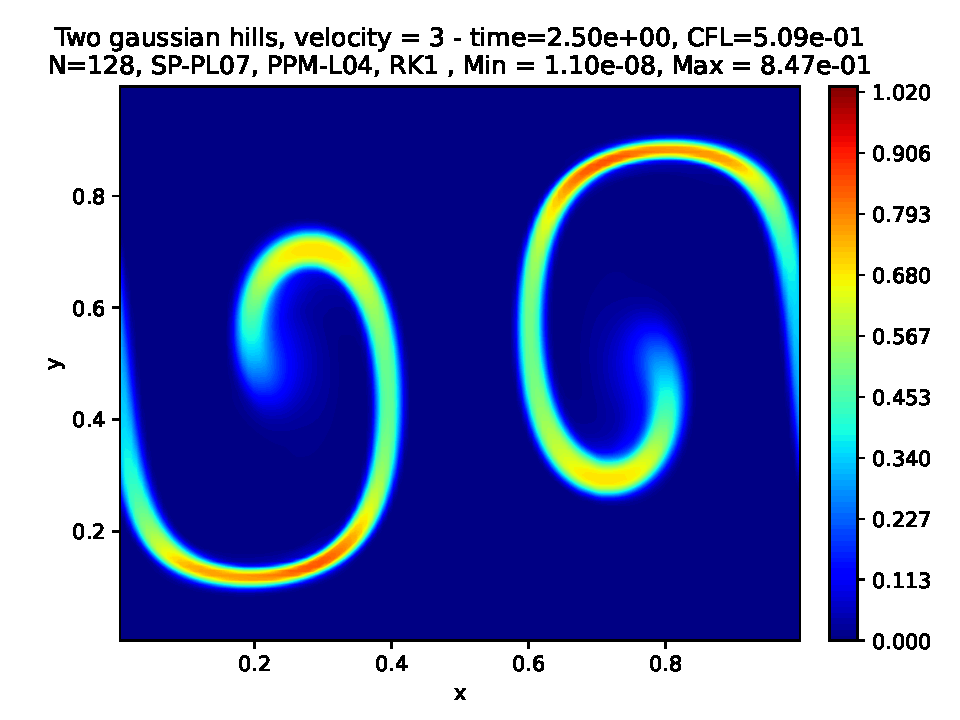
\includegraphics[width=1\linewidth]{2d_adv_tc1_ic4_vf3_t400_N128_SP-PL07_PPM-L04_RK1}
		\caption{PL07 splitting at $t=2.5$.\label{chp3-sec-exp-adv2-e}}
	\end{subfigure}
	\begin{subfigure}{0.4\textwidth}
		\centering
		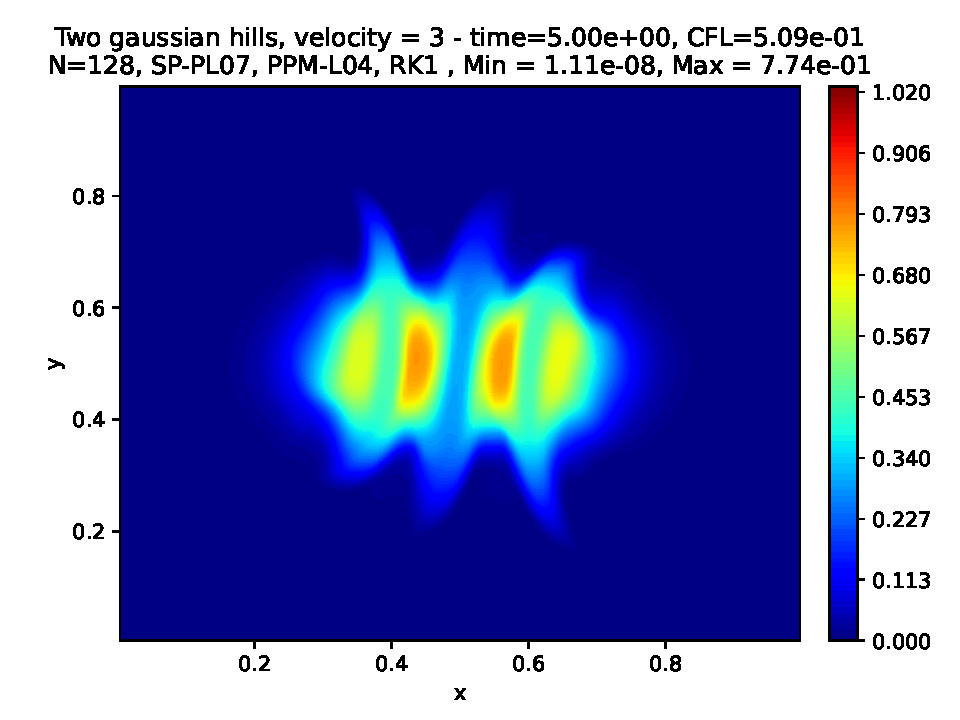
\includegraphics[width=1\linewidth]{2d_adv_tc1_ic4_vf3_t800_N128_SP-PL07_PPM-L04_RK1}
		\caption{PL07 splitting at $t=5$.\label{chp3-sec-exp-adv2-f}}
	\end{subfigure} 
	\caption{Linear advection experiment using the velocity from Equation \eqref{chp3-vf1},
	a CFL number equal to $0.8$, $N=M=128$, and the initial condition is given by Equation \eqref{chp3-ic2}.
	We use the scheme PPM-L04 with AVLT  (\ref{chp3-sec-exp-adv2-a} and \ref{chp3-sec-exp-adv2-b}),
    L04 (\ref{chp3-sec-exp-adv2-c} and \ref{chp3-sec-exp-adv2-d}) and PL07 
    (\ref{chp3-sec-exp-adv2-e} and \ref{chp3-sec-exp-adv2-f}) splitting and RK1 departure point scheme.
	These figures show the advected profile after 2.5 (left) and 5  (right) time units (one time period).
	\label{chp3-sec-exp-adv2}}	
\end{figure}

\begin{figure}[!htb]
	\centering
	\begin{subfigure}{0.42\textwidth}
		\centering
		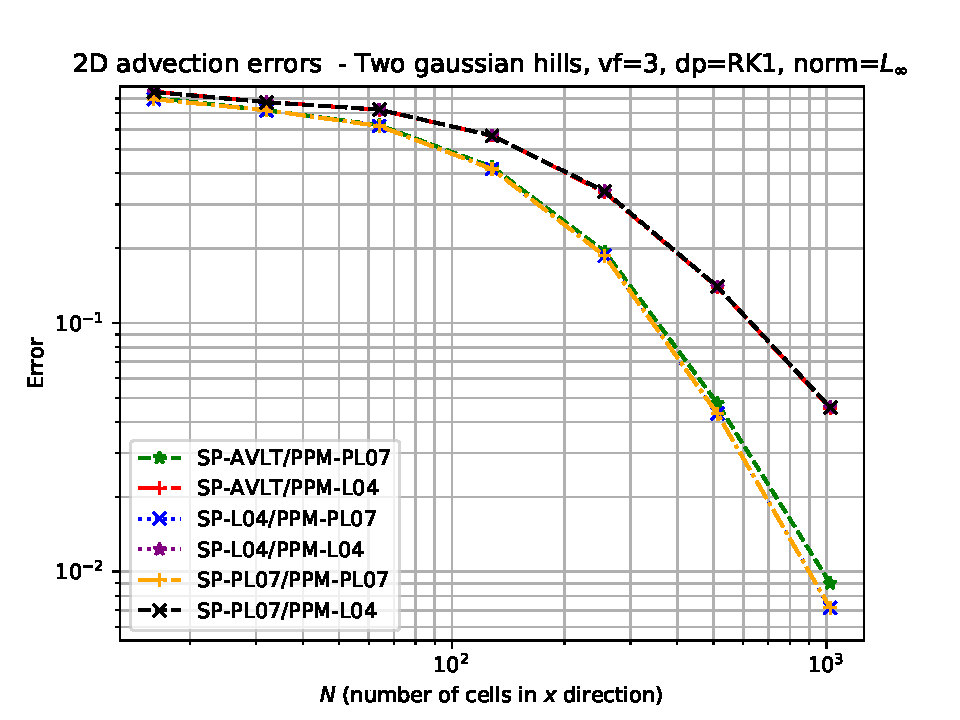
\includegraphics[width=1\linewidth]{2d_adv_tc2_ic4_vf3_dpRK1_normlinf_parabola_errors}
		\caption{RK1.\label{chp3-sec-exp-adv2-error1}}
	\end{subfigure}
	\begin{subfigure}{0.42\textwidth}
		\centering
		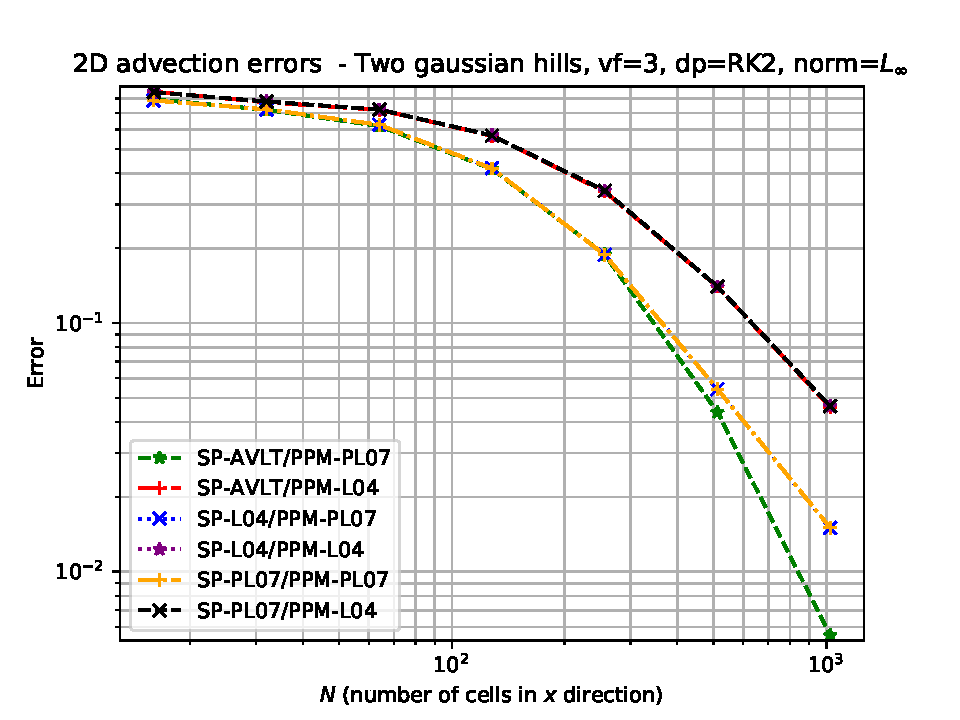
\includegraphics[width=1\linewidth]{2d_adv_tc2_ic4_vf3_dpRK2_normlinf_parabola_errors}
		\caption{RK2.\label{chp3-sec-exp-adv2-error2}}
	\end{subfigure}
	\caption{Convergence of the error for the schemes
	PPM-PL07and PPM-L04 with AVLT/L04/PL07/ splitting
	applied to the linear advection problem using a velocity from Equation \eqref{chp3-vf1},
	a CFL number equal to $0.8$, a final time of integration equal to 5 time units
	and the initial condition given by Equation \eqref{chp3-ic1}.
	The departure points are computed using the RK1 (left) and RK2 (right) schemes.\label{chp3-sec-exp-adv2-error}}
\end{figure}

\begin{figure}[!htb]
	\centering
	\begin{subfigure}{0.42\textwidth}
		\centering
		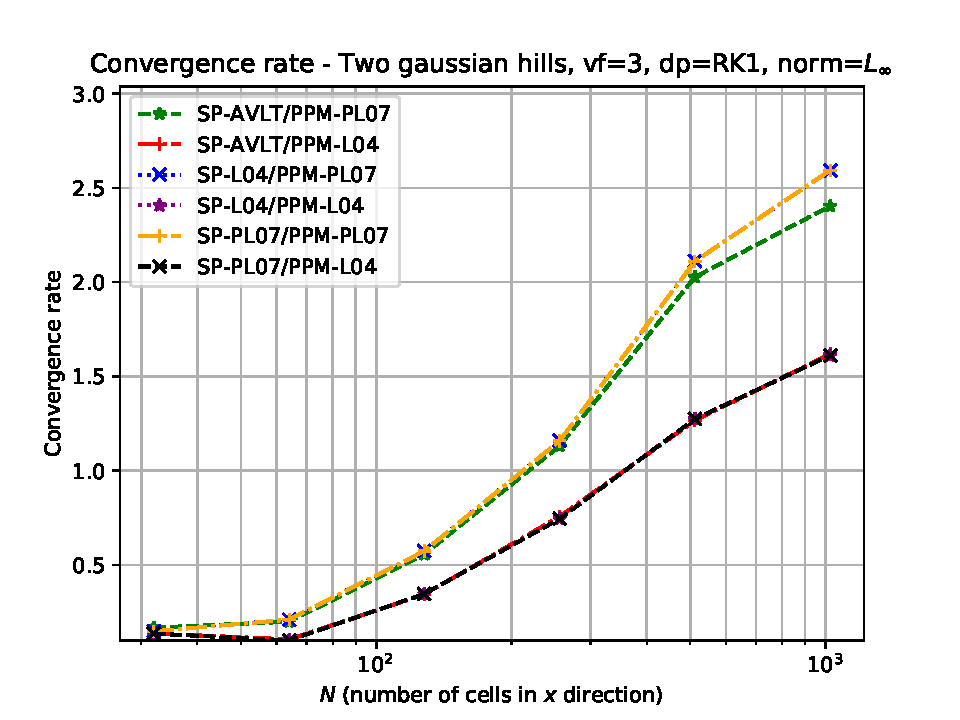
\includegraphics[width=1\linewidth]{2d_adv_tc2_ic4_vf3_dpRK1_normlinf_convergence_rate}
		\caption{RK1.\label{chp3-sec-exp-adv2-cr1}}
	\end{subfigure}
	\begin{subfigure}{0.42\textwidth}
		\centering
		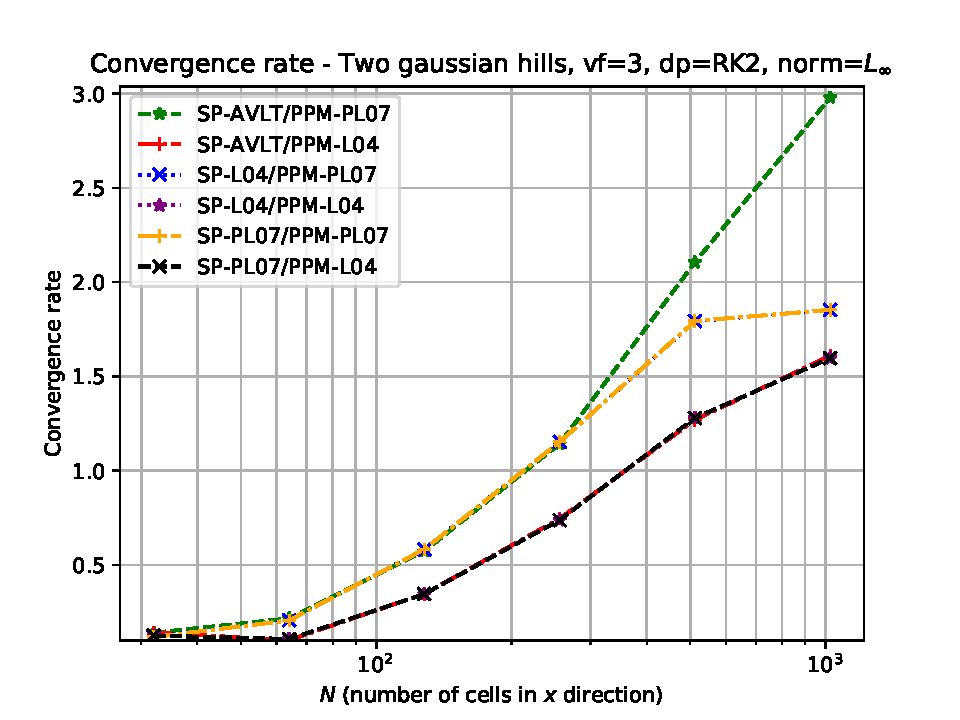
\includegraphics[width=1\linewidth]{2d_adv_tc2_ic4_vf3_dpRK2_normlinf_convergence_rate}
		\caption{RK2.\label{chp3-sec-exp-adv2-cr2}}
	\end{subfigure}
	\caption{Similar to Figure \ref{chp3-sec-exp-adv2-error} but considering the convergence rate.\label{chp3-sec-exp-adv2-cr}}
\end{figure}

\section{Concluding remarks}
In this chapter, we introduced the dimension-splitting method, 
which replaces the solution of the 2D advection equation with the
solution of multiple 1D advection equations, resulting in more cost-effective 2D-FV schemes. 
For our simulations, we adopted the 1D FV-SL scheme based on PPM to solve the 1D equations.

We modified the average of two Lie-Trotter splittings, which is second-order accurate,
to ensure the preservation of a constant scalar field with a divergence-free velocity.
This modification addresses the limitation of the classical averaging
Lie-Trotter splitting and follows the methodology used in FV3.

Based on the simulation with constant velocity, we concluded that all the splitting schemes
are equivalent and do not introduce any splitting errors. In fact, the splittings are exact in this case.
We observed that all the conclusions from the 1D simulations hold true in the 2D case as well,
with mass conservation and monotonicity being preserved when using the monotonic limiters in the 1D subproblems.

In the simulation with variable velocity, we conducted a flow deformation test case.
We observed that all splitting schemes preserved monotonicity in all simulations.
The PL07 and L04 schemes yielded very similar results and introduced a first-order error,
which was observed when using the RK2 scheme to compute the departure point.
Surprisingly, the AVLT scheme achieved third-order accuracy, surpassing its expected second-order accuracy.
This indicates that a more accurate departure point calculation benefits the AVLT splitting.
However, when using a first-order departure point computation, the splitting schemes PL07 and L04 produced slightly smaller errors.
